% Options for packages loaded elsewhere
\PassOptionsToPackage{unicode}{hyperref}
\PassOptionsToPackage{hyphens}{url}
%
\documentclass[
]{article}
\usepackage{amsmath,amssymb}
\usepackage{lmodern}
\usepackage{iftex}
\ifPDFTeX
  \usepackage[T1]{fontenc}
  \usepackage[utf8]{inputenc}
  \usepackage{textcomp} % provide euro and other symbols
\else % if luatex or xetex
  \usepackage{unicode-math}
  \defaultfontfeatures{Scale=MatchLowercase}
  \defaultfontfeatures[\rmfamily]{Ligatures=TeX,Scale=1}
\fi
% Use upquote if available, for straight quotes in verbatim environments
\IfFileExists{upquote.sty}{\usepackage{upquote}}{}
\IfFileExists{microtype.sty}{% use microtype if available
  \usepackage[]{microtype}
  \UseMicrotypeSet[protrusion]{basicmath} % disable protrusion for tt fonts
}{}
\makeatletter
\@ifundefined{KOMAClassName}{% if non-KOMA class
  \IfFileExists{parskip.sty}{%
    \usepackage{parskip}
  }{% else
    \setlength{\parindent}{0pt}
    \setlength{\parskip}{6pt plus 2pt minus 1pt}}
}{% if KOMA class
  \KOMAoptions{parskip=half}}
\makeatother
\usepackage{xcolor}
\usepackage[margin=1in]{geometry}
\usepackage{color}
\usepackage{fancyvrb}
\newcommand{\VerbBar}{|}
\newcommand{\VERB}{\Verb[commandchars=\\\{\}]}
\DefineVerbatimEnvironment{Highlighting}{Verbatim}{commandchars=\\\{\}}
% Add ',fontsize=\small' for more characters per line
\usepackage{framed}
\definecolor{shadecolor}{RGB}{248,248,248}
\newenvironment{Shaded}{\begin{snugshade}}{\end{snugshade}}
\newcommand{\AlertTok}[1]{\textcolor[rgb]{0.94,0.16,0.16}{#1}}
\newcommand{\AnnotationTok}[1]{\textcolor[rgb]{0.56,0.35,0.01}{\textbf{\textit{#1}}}}
\newcommand{\AttributeTok}[1]{\textcolor[rgb]{0.77,0.63,0.00}{#1}}
\newcommand{\BaseNTok}[1]{\textcolor[rgb]{0.00,0.00,0.81}{#1}}
\newcommand{\BuiltInTok}[1]{#1}
\newcommand{\CharTok}[1]{\textcolor[rgb]{0.31,0.60,0.02}{#1}}
\newcommand{\CommentTok}[1]{\textcolor[rgb]{0.56,0.35,0.01}{\textit{#1}}}
\newcommand{\CommentVarTok}[1]{\textcolor[rgb]{0.56,0.35,0.01}{\textbf{\textit{#1}}}}
\newcommand{\ConstantTok}[1]{\textcolor[rgb]{0.00,0.00,0.00}{#1}}
\newcommand{\ControlFlowTok}[1]{\textcolor[rgb]{0.13,0.29,0.53}{\textbf{#1}}}
\newcommand{\DataTypeTok}[1]{\textcolor[rgb]{0.13,0.29,0.53}{#1}}
\newcommand{\DecValTok}[1]{\textcolor[rgb]{0.00,0.00,0.81}{#1}}
\newcommand{\DocumentationTok}[1]{\textcolor[rgb]{0.56,0.35,0.01}{\textbf{\textit{#1}}}}
\newcommand{\ErrorTok}[1]{\textcolor[rgb]{0.64,0.00,0.00}{\textbf{#1}}}
\newcommand{\ExtensionTok}[1]{#1}
\newcommand{\FloatTok}[1]{\textcolor[rgb]{0.00,0.00,0.81}{#1}}
\newcommand{\FunctionTok}[1]{\textcolor[rgb]{0.00,0.00,0.00}{#1}}
\newcommand{\ImportTok}[1]{#1}
\newcommand{\InformationTok}[1]{\textcolor[rgb]{0.56,0.35,0.01}{\textbf{\textit{#1}}}}
\newcommand{\KeywordTok}[1]{\textcolor[rgb]{0.13,0.29,0.53}{\textbf{#1}}}
\newcommand{\NormalTok}[1]{#1}
\newcommand{\OperatorTok}[1]{\textcolor[rgb]{0.81,0.36,0.00}{\textbf{#1}}}
\newcommand{\OtherTok}[1]{\textcolor[rgb]{0.56,0.35,0.01}{#1}}
\newcommand{\PreprocessorTok}[1]{\textcolor[rgb]{0.56,0.35,0.01}{\textit{#1}}}
\newcommand{\RegionMarkerTok}[1]{#1}
\newcommand{\SpecialCharTok}[1]{\textcolor[rgb]{0.00,0.00,0.00}{#1}}
\newcommand{\SpecialStringTok}[1]{\textcolor[rgb]{0.31,0.60,0.02}{#1}}
\newcommand{\StringTok}[1]{\textcolor[rgb]{0.31,0.60,0.02}{#1}}
\newcommand{\VariableTok}[1]{\textcolor[rgb]{0.00,0.00,0.00}{#1}}
\newcommand{\VerbatimStringTok}[1]{\textcolor[rgb]{0.31,0.60,0.02}{#1}}
\newcommand{\WarningTok}[1]{\textcolor[rgb]{0.56,0.35,0.01}{\textbf{\textit{#1}}}}
\usepackage{graphicx}
\makeatletter
\def\maxwidth{\ifdim\Gin@nat@width>\linewidth\linewidth\else\Gin@nat@width\fi}
\def\maxheight{\ifdim\Gin@nat@height>\textheight\textheight\else\Gin@nat@height\fi}
\makeatother
% Scale images if necessary, so that they will not overflow the page
% margins by default, and it is still possible to overwrite the defaults
% using explicit options in \includegraphics[width, height, ...]{}
\setkeys{Gin}{width=\maxwidth,height=\maxheight,keepaspectratio}
% Set default figure placement to htbp
\makeatletter
\def\fps@figure{htbp}
\makeatother
\setlength{\emergencystretch}{3em} % prevent overfull lines
\providecommand{\tightlist}{%
  \setlength{\itemsep}{0pt}\setlength{\parskip}{0pt}}
\setcounter{secnumdepth}{-\maxdimen} % remove section numbering
\ifLuaTeX
  \usepackage{selnolig}  % disable illegal ligatures
\fi
\IfFileExists{bookmark.sty}{\usepackage{bookmark}}{\usepackage{hyperref}}
\IfFileExists{xurl.sty}{\usepackage{xurl}}{} % add URL line breaks if available
\urlstyle{same} % disable monospaced font for URLs
\hypersetup{
  pdftitle={SMI205 Replication Project (2023)},
  pdfauthor={200382007},
  hidelinks,
  pdfcreator={LaTeX via pandoc}}

\title{SMI205 Replication Project (2023)}
\author{200382007}
\date{2023-05-31}

\begin{document}
\maketitle

{
\setcounter{tocdepth}{2}
\tableofcontents
}
\hypertarget{a-multilevel-analysis-of-the-influence-of-lgbt-activism-in-bosnia-and-herzegovina}{%
\section{A Multilevel Analysis of the Influence of LGBT+ Activism in
Bosnia and
Herzegovina}\label{a-multilevel-analysis-of-the-influence-of-lgbt-activism-in-bosnia-and-herzegovina}}

\hypertarget{rpubs-link-copy-rpubs-url-address-here}{%
\subsubsection{Rpubs link: {[}copy Rpubs url address
here{]}}\label{rpubs-link-copy-rpubs-url-address-here}}

\hypertarget{github-repository-add-url-here-if-you-have-created-a-data-or-code-repository-if-not-delete-this-line}{%
\subsubsection{GitHub Repository: {[}add url here if you have created a
data or code repository, if not delete this
line{]}}\label{github-repository-add-url-here-if-you-have-created-a-data-or-code-repository-if-not-delete-this-line}}

\hypertarget{study-preregistration-form-httpsrpubs.comsn2003820071043913}{%
\subsubsection{\texorpdfstring{Study Preregistration form:
\url{https://rpubs.com/sn200382007/1043913}}{Study Preregistration form: https://rpubs.com/sn200382007/1043913}}\label{study-preregistration-form-httpsrpubs.comsn2003820071043913}}

\hypertarget{information-about-this-replication-project}{%
\subsection{Information about this replication
project}\label{information-about-this-replication-project}}

\begin{itemize}
\tightlist
\item
  Replication project based on paper {[}add full citation here and link
  to its published online version{]}
\item
  Replication method (select one from below):

  \begin{itemize}
  \tightlist
  \item
    Used replication package available at {[}add citation + repository
    link here{]}
  \item
    Used materials obtained from authors
  \item
    Own replication following methods section of the paper
  \item
    Other - explain
  \end{itemize}
\end{itemize}

\hypertarget{workspace-setup}{%
\subsection{Workspace setup}\label{workspace-setup}}

\hypertarget{yaml-settings}{%
\subsubsection{YAML settings}\label{yaml-settings}}

output: ~ html\_document: ~~ code\_download: true ~~~ toc: true ~~~
toc\_depth: 2 ~~~ toc\_float: ~~~~ collapsed: false ~~~~ smooth\_scroll:
true

\hypertarget{global-settings-of-r-chunks}{%
\subsubsection{Global settings of R
chunks}\label{global-settings-of-r-chunks}}

\begin{Shaded}
\begin{Highlighting}[]
\CommentTok{\# Global options}
\NormalTok{opts\_chunk}\SpecialCharTok{$}\FunctionTok{set}\NormalTok{(}\AttributeTok{echo=}\ConstantTok{TRUE}\NormalTok{,}
                 \AttributeTok{cache=}\ConstantTok{TRUE}\NormalTok{,}
               \AttributeTok{comment=}\ConstantTok{NA}\NormalTok{,}
               \AttributeTok{message=}\ConstantTok{FALSE}\NormalTok{,}
               \AttributeTok{warning=}\ConstantTok{FALSE}\NormalTok{)}
\end{Highlighting}
\end{Shaded}

\hypertarget{libraries}{%
\subsubsection{Libraries}\label{libraries}}

\begin{Shaded}
\begin{Highlighting}[]
\CommentTok{\#general}
\FunctionTok{library}\NormalTok{(tidyverse)}

\CommentTok{\#data cleaning}
\FunctionTok{library}\NormalTok{(stringi)}

\CommentTok{\#for maps}
\FunctionTok{library}\NormalTok{(sf)}
\FunctionTok{library}\NormalTok{(geojsonsf)}
\FunctionTok{library}\NormalTok{(ggpubr)}

\CommentTok{\#for modelling}
\FunctionTok{library}\NormalTok{(lme4)}
\FunctionTok{library}\NormalTok{(haven)}
\FunctionTok{library}\NormalTok{(merTools)}
\FunctionTok{library}\NormalTok{(lattice)}

\CommentTok{\#for presenting outputs}
\FunctionTok{library}\NormalTok{(sjPlot)}
\FunctionTok{library}\NormalTok{(glmmTMB)}
\end{Highlighting}
\end{Shaded}

\hypertarget{versions-of-used-packages}{%
\subsubsection{Versions of used
packages}\label{versions-of-used-packages}}

\begin{verbatim}
$rmarkdown
[1] '2.18'

$knitr
[1] '1.41'

$tidyverse
[1] '2.0.0'

$stringi
[1] '1.7.8'

$sf
[1] '1.0.13'

$geojsonsf
[1] '2.0.3'

$ggpubr
[1] '0.6.0'

$lme4
[1] '1.1.31'

$haven
[1] '2.5.2'

$merTools
[1] '0.5.2'

$lattice
[1] '0.20.45'

$sjPlot
[1] '2.8.13'

$glmmTMB
[1] '1.1.5'
\end{verbatim}

\hypertarget{my-enviroment}{%
\subsubsection{My enviroment}\label{my-enviroment}}

\begin{verbatim}
[1] "R version 4.2.3 (2023-03-15)"
\end{verbatim}

\hypertarget{introduction}{%
\subsection{1. Introduction}\label{introduction}}

Ayoub et al.'s paper Pride amidst Prejudice (2020) studied the effect
that the first Pride Parade held in Bosnia and Herzegovina had on
support of LGBT+ people across the country, finding a positive change in
attitude within Sarajevo but no diffusion effect nor backlash in the
rest of the country. I previously conducted a replication using the same
data and same methods to test the paper's verifiability; my results
fully supported the outcomes of the original paper. Although Ayoub et
al.~were interested in studying whether the effect of Pride spread
outside of Sarajevo, they split their linear regression models only by
Sarajevo and rest of Country. This limited the ability to study the
diffusion effect as it grouped municipalities that bordered Sarajevo -
and may have residents who commute into the city thus blurring the
boundaries of the city limits - with municipalities in the furthest
reaches of the country. Additionally, there may be differences in
response within the city of Sarajevo, as the Pride took place only
within the Centar municipality: individuals from other Sarajevo
municipalities could choose to travel to the Pride whereas individuals
within Centar would be affected as the default.

Pride Parades can be an important tool for LGBT+ activists to disrupt
the heteronormative order, increase the community's visibility, and
create a shared community identity. Existing qualitative research has
been conducted primarily within socially liberal, accepting societies,
interviewing attendees on their experiences. Ayoub et al.'s research is
therefore vital to the field as it examines the risk of increasing
visibility within a socially conservative society, allowing us to
determine whether Prides are effective and worth the risk. This
extension of their work will further examine the efficacy of Prides, and
look at how municipal contexts affect an individual's initial attitude
and response to Pride. While the original paper found Pride to have a
positive effect on acceptance within Sarajevo as a whole, a relatively
more negative response within the Centar municipality could suggest a
successful destabilisation of the heteronormative society that would
have allowed LGBT+ individuals to express their own identities among
their communities in a way that antagonised the general public, whereas
a more positive response could indicate the creation of positive
location based memories for those who attended.

With increased visibility comes the risk of heightened intolerance,
which may be particularly the case in Bosnia and Herzegovina. The
country has a strong presence of ethnonationalism and religious
separatism, which political leaders use to their advantage to exacerbate
an `us vs them' attitude. Hadzic et al.~study how a municipality's
collective memory - such as of casualty of the Bosnian Civil War - can
lead to polarising views and high patterns of ethnocentric voting, which
may also affect acceptance of other minority groups such as LGBT+
people, as nationalism rejects competing or alternative identities. In a
study of homophobia experienced within US schools, {[}{]} found
influences from community characteristics such as average levels of
education and religion, showing the effect a community can have on an
individual's attitudes. In this extension, I will investigate how
individuals are affected by characteristics of municipalities, and
whether different individual level factors such as religiosity have the
same effect everywhere or if the effect of an individual characteristic
can vary dependent on the community they're embedded within.

\hypertarget{data-and-methods}{%
\subsection{2. Data and methods}\label{data-and-methods}}

\hypertarget{data}{%
\subsubsection{2.1. Data}\label{data}}

\begin{Shaded}
\begin{Highlighting}[]
\CommentTok{\#Data}
\CommentTok{\#Read data and shapefile}
\NormalTok{rep\_data }\OtherTok{\textless{}{-}} \FunctionTok{read\_dta}\NormalTok{(}\StringTok{\textquotesingle{}Data/Pride\_Amid\_Prejudice\_replication data\_final.dta\textquotesingle{}}\NormalTok{)}
\NormalTok{shape }\OtherTok{\textless{}{-}} \FunctionTok{geojson\_sf}\NormalTok{(}\StringTok{"Data/geoBoundaries{-}BIH{-}ADM2.geojson"}\NormalTok{)}

\CommentTok{\#Remove non{-}Latin characters and macth name discrepencies, eg.}
\NormalTok{shape}\SpecialCharTok{$}\NormalTok{shapeName }\OtherTok{=} \FunctionTok{stri\_trans\_general}\NormalTok{(}\AttributeTok{str =}\NormalTok{ shape}\SpecialCharTok{$}\NormalTok{shapeName, }\AttributeTok{id =} \StringTok{"Latin{-}ASCII"}\NormalTok{)}
\NormalTok{shape[}\DecValTok{15}\NormalTok{, }\StringTok{"shapeName"}\NormalTok{] }\OtherTok{\textless{}{-}} \StringTok{"Bosanska Gradiska (Gradiska)"}
\end{Highlighting}
\end{Shaded}

\begin{Shaded}
\begin{Highlighting}[]
\CommentTok{\#Merge survey data and shapefile}
\NormalTok{rep\_shape }\OtherTok{\textless{}{-}} \FunctionTok{inner\_join}\NormalTok{(rep\_data, shape, }\AttributeTok{by =} \FunctionTok{join\_by}\NormalTok{(}\StringTok{"municipalitystr"} \SpecialCharTok{==} \StringTok{"shapeName"}\NormalTok{))}
\CommentTok{\#Remove observations with missing data}
\NormalTok{rep\_shape\_m }\OtherTok{\textless{}{-}}\NormalTok{ rep\_shape[}\FunctionTok{complete.cases}\NormalTok{(rep\_shape[,}\FunctionTok{c}\NormalTok{(}\StringTok{\textquotesingle{}ethnocentric\textquotesingle{}}\NormalTok{, }\StringTok{\textquotesingle{}religious\textquotesingle{}}\NormalTok{, }\StringTok{\textquotesingle{}Education\textquotesingle{}}\NormalTok{)]),]}
\CommentTok{\#Rescale variables}
\NormalTok{rep\_shape\_m}\SpecialCharTok{$}\NormalTok{vote\_share\_10 }\OtherTok{\textless{}{-}}\NormalTok{ rep\_shape\_m}\SpecialCharTok{$}\NormalTok{ethnic\_vote\_share}\SpecialCharTok{/}\DecValTok{10}
\NormalTok{rep\_shape\_m}\SpecialCharTok{$}\NormalTok{age\_10 }\OtherTok{\textless{}{-}}\NormalTok{ rep\_shape\_m}\SpecialCharTok{$}\NormalTok{age}\SpecialCharTok{/}\DecValTok{10}
\end{Highlighting}
\end{Shaded}

This extension uses the data collected by Ayoub et al.~and provided on
the Harvard Dataverse Repository as part of the replication materials.
The questionnaire and panel data totals to 2,430 respondents after
accounting for initial missingness; these responses are spread across 70
of the 143 total municipalities. The original study made use of some
municipality data provided by Hadzic et al.; I accessed the full Hadzic
dataset but determined there were no further variables that could be
relevant to this study. To assist with spatial analysis of the diffusion
effect, I use shapefile data as provided by the United Nations' Office
for the Coordination of Humanitarian Affairs' Humanitarian Data Exchange
service (Runfola et al., 2020).

The outcome variable is measured on a scale of 1 to 4, where 4 is
strongly support Pride and 1 is strongly oppose. The predictor is a
binary variable for whether the response was from before or after the
Pride event. At Level 1 (individual) are dummies for unemployed, gender
(male), EU vote. Religiosity is measured from 1 to 3 (3 = very
religious). Ethnic identity is recorded as Bosnian, Serb, Croat, or
Bosniak, and recoded as dummies with Bosnian as the reference category.
Education level is measured from 1 to 11, where 3 is left school at 15
and 11 indicates a doctorate. I have recoded age to one tenth of its
original value to aid with interpretation, so 56 years old becomes 5.6.
At Level 2 (municipality) I have recoded ethnic vote share from a
percentage to 0 to 10, where 56\% = 5.6. Casualty is the proportion of
the municipality population dead or missing following the Bosnian Civil
War as a measure of experience of wartime violence.

In order to combine the survey data with the shapefile I replaced all
non Latin characters in municipality names then combed through to find
and rename discrepancies (e.g.~``Bosnanska Gradiška/Gradiška'' became
``Bosanska Gradiska (Gradiska)''); this allowed the two datasets to be
merged by matching municipality names. I then omitted observations that
missed data for any of the variables I was using in my models, leaving
me with 2,343 total observations.

\#insert some maps, descriptive statistics, code snippets

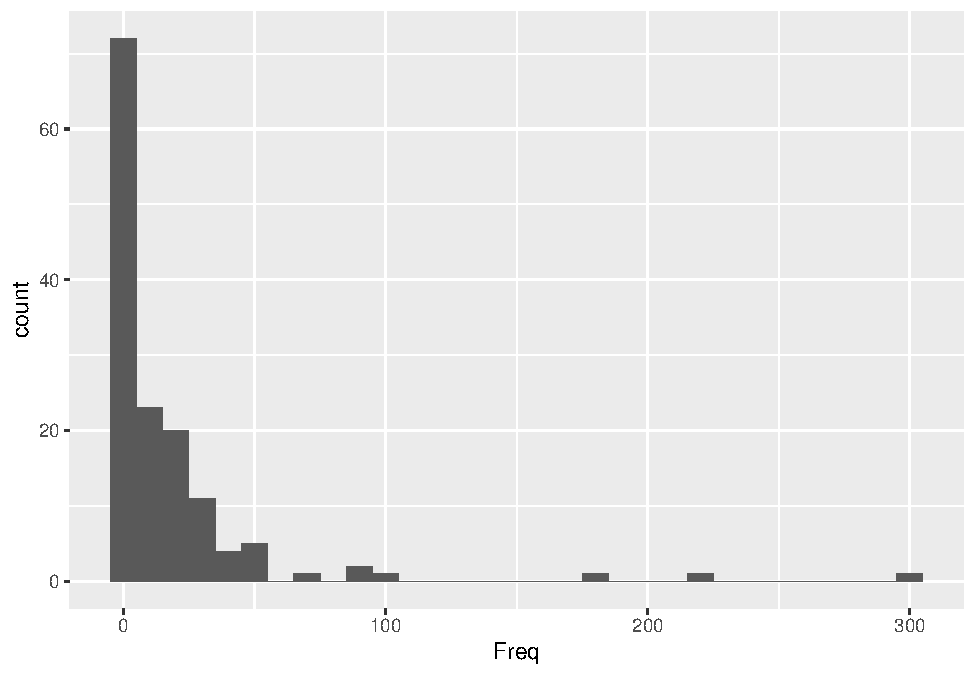
\includegraphics{SMI205_Assessment2_Template_files/figure-latex/distributions plots-1.pdf}
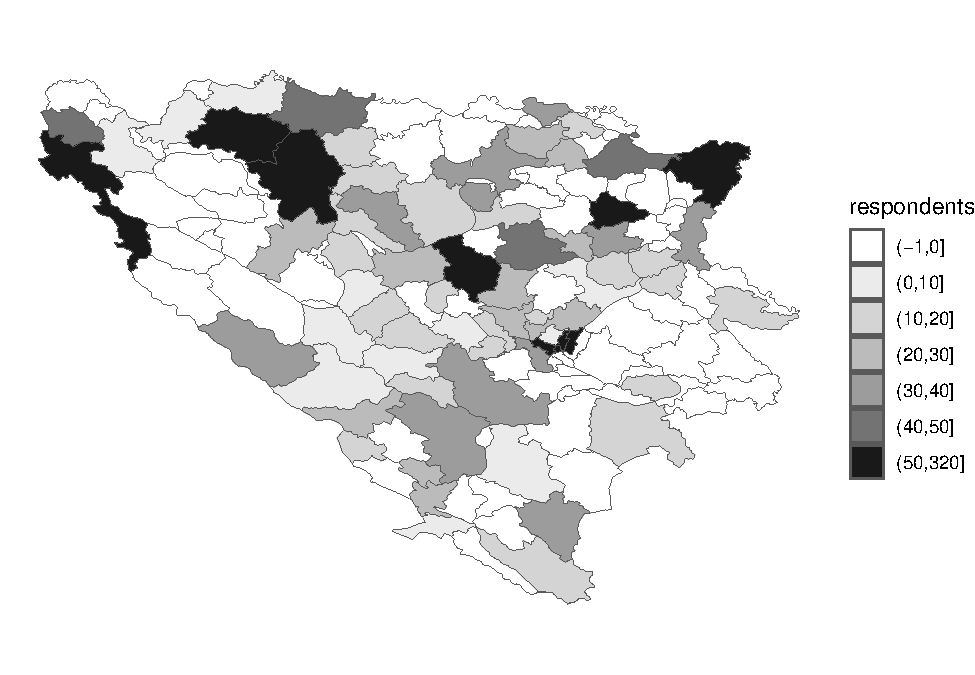
\includegraphics{SMI205_Assessment2_Template_files/figure-latex/distributions plots-2.pdf}

\hypertarget{methods}{%
\subsubsection{2.2. Methods}\label{methods}}

This extension is a test the robustness of the original paper's findings
as I am using the same data but different methods. Whereas Ayoub et
al.~used single level ordinary least squares regression and compared
models for within Sarajevo and the rest of the country, I am using a two
level random slopes model. This allows for the full range of
sociodemographic variables to be considered at L1 alongside L2 variables
about the municipality overall. I begin with a null model and add
variables individually, removing ones that are not statistically
significant. When adding each L1 variable I will also test whether it
fits better as a fixed or random effect, using AIC and Anova tests to
determine comparative fit. Testing variables for random effects is
important to understand how a community may affect how an individual's
characteristic may influence them. For example, a the religiosity of an
individual in a municipality with inclusive churches and mosques may
have a different affect on them compared to if they lived in a community
with strictly orthodox religions. The two level model is also useful to
examine whether the effect of holding the Pride event diffused across
the country or was seen only within Sarajevo - if at all. It also allows
us to identify other cities which may be contextually more similar to
Sarajevo and analyse whether they responded in a similar way or whether
the effect was indeed geographically centred around the Pride. Allowing
slopes to be random means we can see which municipalities became more
supportive (reacted positively) and which saw backlash (reacted
negatively). The grouping used in the original study found that overall
Sarajevo started most supportive and became even more so, whereas the
rest of the country saw minimal effect. This obscures positive responses
across the rest of the country as well as variation within Sarajevo; if
the pattern of the most supportive becoming even more so holds outside
of Sarajevo, then it is possible that there may be some fanning out
where the least supportive react negatively which could help identify
possible areas for backlash.

\#insert code snippers of models, comparison tests

\begin{Shaded}
\begin{Highlighting}[]
\DocumentationTok{\#\#\#random slopes models}
\NormalTok{slopes.m }\OtherTok{\textless{}{-}} \FunctionTok{lmer}\NormalTok{(supportpride }\SpecialCharTok{\textasciitilde{}}\NormalTok{ treatment }\SpecialCharTok{+}\NormalTok{ (}\DecValTok{1} \SpecialCharTok{+}\NormalTok{ treatment}\SpecialCharTok{|}\NormalTok{municipalitystr), }\AttributeTok{data =}\NormalTok{ rep\_shape\_m, }\AttributeTok{na.action=}\StringTok{"na.exclude"}\NormalTok{)}
\end{Highlighting}
\end{Shaded}

\begin{verbatim}
Linear mixed model fit by REML ['lmerMod']
Formula: supportpride ~ treatment + (1 + treatment | municipalitystr)
   Data: rep_shape_m

REML criterion at convergence: 5717.5

Scaled residuals: 
    Min      1Q  Median      3Q     Max 
-1.7038 -0.5947 -0.3235  0.5845  2.8932 

Random effects:
 Groups          Name        Variance Std.Dev. Corr
 municipalitystr (Intercept) 0.090176 0.30029      
                 treatment   0.001568 0.03959  1.00
 Residual                    0.813000 0.90167      
Number of obs: 2136, groups:  municipalitystr, 70

Fixed effects:
            Estimate Std. Error t value
(Intercept)  1.50267    0.04853  30.964
treatment    0.03777    0.04044   0.934

Correlation of Fixed Effects:
          (Intr)
treatment -0.310
\end{verbatim}

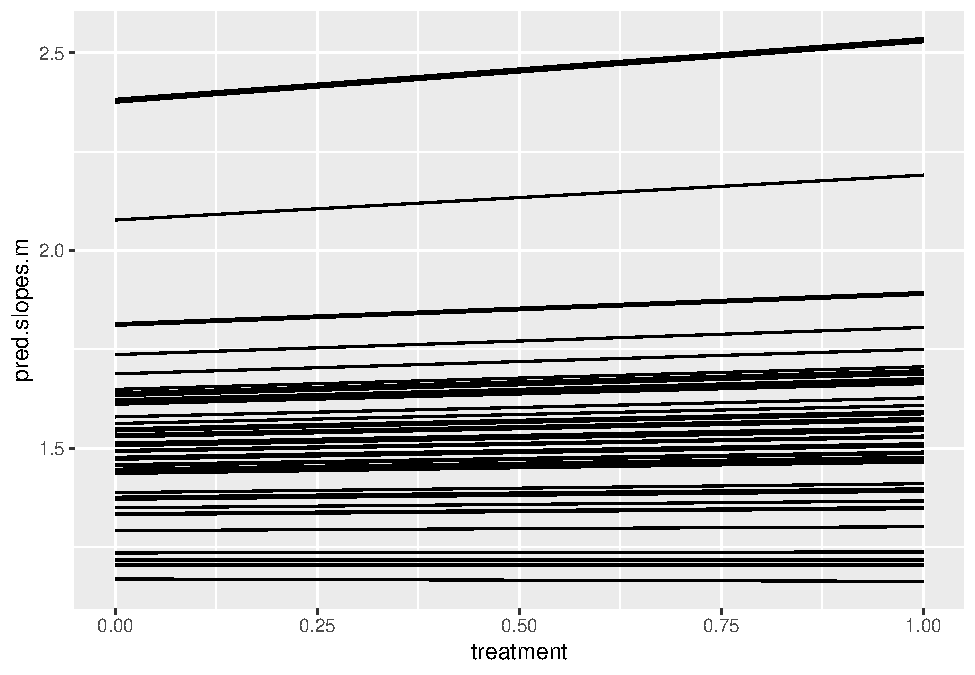
\includegraphics{SMI205_Assessment2_Template_files/figure-latex/random slopes plots-1.pdf}

\begin{verbatim}
$municipalitystr
\end{verbatim}

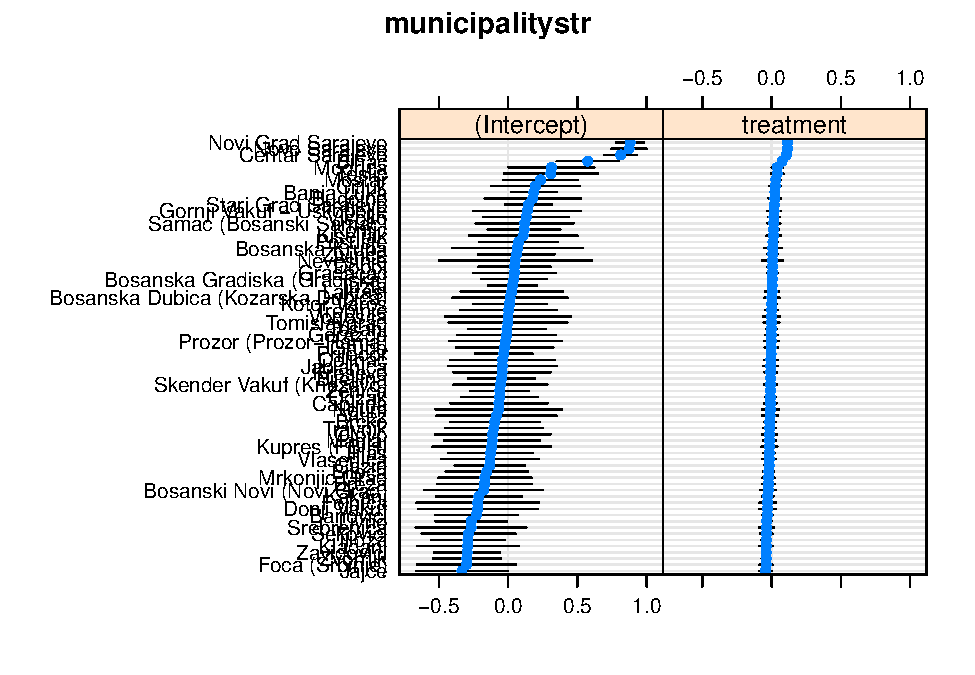
\includegraphics{SMI205_Assessment2_Template_files/figure-latex/random slopes plots-2.pdf}
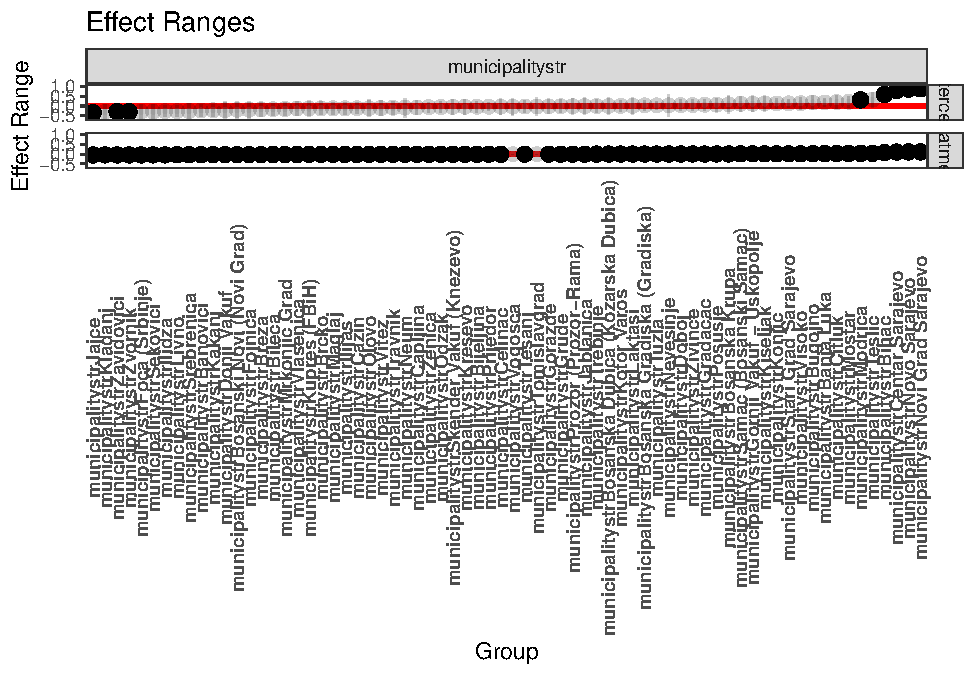
\includegraphics{SMI205_Assessment2_Template_files/figure-latex/random slopes plots-3.pdf}

\begin{Shaded}
\begin{Highlighting}[]
\CommentTok{\#Example of testing for random effects}
\NormalTok{(slopes}\FloatTok{.4}\NormalTok{a }\OtherTok{\textless{}{-}} \FunctionTok{lmer}\NormalTok{(supportpride }\SpecialCharTok{\textasciitilde{}}\NormalTok{ treatment }\SpecialCharTok{+}\NormalTok{ unemployed }\SpecialCharTok{+}\NormalTok{ Men }\SpecialCharTok{+}\NormalTok{ voteeu }\SpecialCharTok{+}\NormalTok{ ethnocentric }\SpecialCharTok{+}\NormalTok{ (}\DecValTok{1} \SpecialCharTok{+}\NormalTok{ treatment}\SpecialCharTok{|}\NormalTok{municipalitystr),}
                   \AttributeTok{data =}\NormalTok{ rep\_shape\_m, }\AttributeTok{na.action=}\StringTok{"na.exclude"}\NormalTok{))}
\end{Highlighting}
\end{Shaded}

\begin{verbatim}
Linear mixed model fit by REML ['lmerMod']
Formula: supportpride ~ treatment + unemployed + Men + voteeu + ethnocentric +  
    (1 + treatment | municipalitystr)
   Data: rep_shape_m
REML criterion at convergence: 5651.542
Random effects:
 Groups          Name        Std.Dev. Corr
 municipalitystr (Intercept) 0.28820      
                 treatment   0.03716  1.00
 Residual                    0.88551      
Number of obs: 2136, groups:  municipalitystr, 70
Fixed Effects:
 (Intercept)     treatment    unemployed           Men        voteeu  
     1.59563       0.06389      -0.11952      -0.06958       0.17616  
ethnocentric  
    -0.32872  
optimizer (nloptwrap) convergence code: 0 (OK) ; 0 optimizer warnings; 1 lme4 warnings 
\end{verbatim}

\begin{Shaded}
\begin{Highlighting}[]
\NormalTok{(slopes}\FloatTok{.4}\NormalTok{b }\OtherTok{\textless{}{-}} \FunctionTok{lmer}\NormalTok{(supportpride }\SpecialCharTok{\textasciitilde{}}\NormalTok{ treatment }\SpecialCharTok{+}\NormalTok{ unemployed }\SpecialCharTok{+}\NormalTok{ Men }\SpecialCharTok{+}\NormalTok{ voteeu }\SpecialCharTok{+}\NormalTok{ ethnocentric }\SpecialCharTok{+}\NormalTok{ (}\DecValTok{1} \SpecialCharTok{+}\NormalTok{ treatment }\SpecialCharTok{+}\NormalTok{ ethnocentric}\SpecialCharTok{|}\NormalTok{municipalitystr),}
                   \AttributeTok{data =}\NormalTok{ rep\_shape\_m, }\AttributeTok{na.action=}\StringTok{"na.exclude"}\NormalTok{))}
\end{Highlighting}
\end{Shaded}

\begin{verbatim}
Linear mixed model fit by REML ['lmerMod']
Formula: supportpride ~ treatment + unemployed + Men + voteeu + ethnocentric +  
    (1 + treatment + ethnocentric | municipalitystr)
   Data: rep_shape_m
REML criterion at convergence: 5603.242
Random effects:
 Groups          Name         Std.Dev. Corr       
 municipalitystr (Intercept)  0.3835              
                 treatment    0.0801    0.56      
                 ethnocentric 0.2125   -1.00 -0.52
 Residual                     0.8750              
Number of obs: 2136, groups:  municipalitystr, 70
Fixed Effects:
 (Intercept)     treatment    unemployed           Men        voteeu  
     1.50309       0.03860      -0.11986      -0.06522       0.17654  
ethnocentric  
    -0.15608  
optimizer (nloptwrap) convergence code: 0 (OK) ; 0 optimizer warnings; 1 lme4 warnings 
\end{verbatim}

\begin{Shaded}
\begin{Highlighting}[]
\FunctionTok{anova}\NormalTok{(slopes}\FloatTok{.4}\NormalTok{b, slopes}\FloatTok{.4}\NormalTok{a) }\CommentTok{\#4b better, effect of ethnocentrism varies by municipality}
\end{Highlighting}
\end{Shaded}

\begin{verbatim}
Data: rep_shape_m
Models:
slopes.4a: supportpride ~ treatment + unemployed + Men + voteeu + ethnocentric + (1 + treatment | municipalitystr)
slopes.4b: supportpride ~ treatment + unemployed + Men + voteeu + ethnocentric + (1 + treatment + ethnocentric | municipalitystr)
          npar    AIC    BIC  logLik deviance Chisq Df Pr(>Chisq)    
slopes.4a   10 5645.1 5701.7 -2812.5   5625.1                        
slopes.4b   13 5602.8 5676.5 -2788.4   5576.8 48.26  3  1.874e-10 ***
---
Signif. codes:  0 '***' 0.001 '**' 0.01 '*' 0.05 '.' 0.1 ' ' 1
\end{verbatim}

\begin{Shaded}
\begin{Highlighting}[]
\FunctionTok{summary}\NormalTok{(slopes}\FloatTok{.4}\NormalTok{b) }\CommentTok{\#is the effect significant?}
\end{Highlighting}
\end{Shaded}

\begin{verbatim}
Linear mixed model fit by REML ['lmerMod']
Formula: supportpride ~ treatment + unemployed + Men + voteeu + ethnocentric +  
    (1 + treatment + ethnocentric | municipalitystr)
   Data: rep_shape_m

REML criterion at convergence: 5603.2

Scaled residuals: 
    Min      1Q  Median      3Q     Max 
-2.1888 -0.6257 -0.3076  0.5725  3.0314 

Random effects:
 Groups          Name         Variance Std.Dev. Corr       
 municipalitystr (Intercept)  0.147085 0.3835              
                 treatment    0.006416 0.0801    0.56      
                 ethnocentric 0.045177 0.2125   -1.00 -0.52
 Residual                     0.765649 0.8750              
Number of obs: 2136, groups:  municipalitystr, 70

Fixed effects:
             Estimate Std. Error t value
(Intercept)   1.50309    0.07606  19.763
treatment     0.03860    0.04179   0.924
unemployed   -0.11986    0.04983  -2.406
Men          -0.06522    0.03872  -1.684
voteeu        0.17654    0.04906   3.599
ethnocentric -0.15608    0.05192  -3.006

Correlation of Fixed Effects:
            (Intr) trtmnt unmply Men    voteeu
treatment   -0.090                            
unemployed  -0.157  0.031                     
Men         -0.224 -0.022  0.029              
voteeu      -0.485 -0.082 -0.007 -0.036       
ethnocentrc -0.655 -0.150  0.028  0.023  0.039
optimizer (nloptwrap) convergence code: 0 (OK)
boundary (singular) fit: see help('isSingular')
\end{verbatim}

\begin{Shaded}
\begin{Highlighting}[]
\FunctionTok{anova}\NormalTok{(slopes}\FloatTok{.3}\NormalTok{a, slopes}\FloatTok{.4}\NormalTok{b) }\CommentTok{\#better than the earlier model}
\end{Highlighting}
\end{Shaded}

\begin{verbatim}
Data: rep_shape_m
Models:
slopes.3a: supportpride ~ treatment + unemployed + Men + voteeu + (1 + treatment | municipalitystr)
slopes.4b: supportpride ~ treatment + unemployed + Men + voteeu + ethnocentric + (1 + treatment + ethnocentric | municipalitystr)
          npar    AIC    BIC  logLik deviance  Chisq Df Pr(>Chisq)    
slopes.3a    9 5705.0 5756.0 -2843.5   5687.0                         
slopes.4b   13 5602.8 5676.5 -2788.4   5576.8 110.17  4  < 2.2e-16 ***
---
Signif. codes:  0 '***' 0.001 '**' 0.01 '*' 0.05 '.' 0.1 ' ' 1
\end{verbatim}

\begin{Shaded}
\begin{Highlighting}[]
\NormalTok{slopes.final }\OtherTok{\textless{}{-}} \FunctionTok{lmer}\NormalTok{(supportpride }\SpecialCharTok{\textasciitilde{}}\NormalTok{ treatment }\SpecialCharTok{+}\NormalTok{ unemployed }\SpecialCharTok{+}\NormalTok{ Men }\SpecialCharTok{+}\NormalTok{ voteeu }\SpecialCharTok{+}\NormalTok{ ethnocentric }\SpecialCharTok{+} 
\NormalTok{                       religious }\SpecialCharTok{+}\NormalTok{ Bosniak }\SpecialCharTok{+}\NormalTok{ Education }\SpecialCharTok{+}\NormalTok{ vote\_share\_10 }\SpecialCharTok{+} 
\NormalTok{                        (}\DecValTok{1} \SpecialCharTok{+}\NormalTok{ treatment }\SpecialCharTok{+}\NormalTok{ ethnocentric }\SpecialCharTok{+}\NormalTok{ religious}\SpecialCharTok{|}\NormalTok{municipalitystr),}
                           \AttributeTok{data =}\NormalTok{ rep\_shape\_m, }\AttributeTok{na.action=}\StringTok{"na.exclude"}\NormalTok{)}
\end{Highlighting}
\end{Shaded}

\hypertarget{results}{%
\subsection{3. Results}\label{results}}

The final model found that while some of the L2 random effects were
significant, the effect of Pride on support for LGBT+ people across the
country was not significant. The random effects on the intercept show
that Zavdovici and Ilidza are significantly less supportive of LGBT+
people, whereas the Sarajevo municipalities of Novo, Centar, and Novi
Grad - as well as Teslic and Bihac - are significantly more supportive
of Pride to begin with. Interestingly, the fourth Sarajevo municipality,
Stari Grad, was more negative than average, although this was not
statistically significant. The random effects of treatment (pre vs post
Pride) appeared to `fan out', and a Pearson's correlation test showed a
positive relationship between intercept and treatment meaning more
accepting municipalities responded more positively while some
unsupportive municipalities reacted negatively. No conclusions can be
drawn from this, however, as Pride occurring (treatment) was not found
to be statistically significant at the 95\% level.

Both ethnocentrism and religiosity were found to be significant as
random effects, showing that religious and ethnic communities are not
monolithic but their effect on individuals varies by municipality.
Further research could be completed to uncover what factors within
religious communities cause these differences as most existing research
finds that increased religiosity decreases acceptance of LGBT+ people.

In terms of fixed effects, being unemployed and being a male each
decreased support for LGBT+ people (measured from 1-4) by 0.11. This
aligns with literature around how radicalisation and nationalism take
advantage of unemployment to pass blame and stoke an `us vs them'
rhetoric, while also promoting ideas of patriarchy and family structure.
Following on from this, voting in favour of the EU was associated with
being 0.19 more supportive; this corresponds with studies of the social
changes that post-Soviet and post-Yugoslav societies have undergone
before joining the EU as hosting a Pride event is commonly observed to
be a major step towards this. Another indicator of being more receptive
to LGBT+ people was education: with each further level of education
achieved, individuals were 0.07 more supportive, meaning someone with a
doctorate (coded as 11) was on average 0.56 more supportive than someone
who left school at 15 (after primary education, coded as 3). In the
other direction, Bosniaks were found to be 0.35 less supportive than
Bosnians as the reference category, but Croats and Serbs were not found
to differ significantly in support compared to Bosnians. Finally, the
fixed effect of ethnic vote share found that for every extra 10\% of the
municipality vote went to ethnonationalist parties, individuals within
that municipality were 0.11 less supportive (eg. in a municipality with
80\% ethnic vote share individuals will be an estimated 0.33 less
supportive than in a municipality with 50\% ethnic vote). This is backed
up by {[}Hadzic, Swimelar{]} who document how nationalist politicians
use LGBT+ issues as an enemy to unite against and gain legitimacy by
claiming to defend the national identity that LGBT+ people would
purportedly undermine.

In making this model, several variables were tested but found not to
have a significant effect. Age was not found to have a significant
effect on support for LGBT+ people, which contrasts to the findings of
the original paper. This may be due to demographic changes such as
increased education, reduced religiosity or ethnocentrism that may be
prevalent among younger people and account for any difference in support
found. It may also be accounted for by municipality, as young supportive
people may relocate to cities for work and opportunities, so effects may
get absorbed by other variables. Population density was not found to be
significant which was somewhat surprising as theories around
socialisation tend to find that the more exposure to different people
one has, the more inclusive one is compared to those in sparsely
populated regions who may be isolated or part of insulated communities.
Level of casualty as studied by Hadzic was not found to have a direct
effect on acceptance, though it may still indirectly have an effect as
Hadzic found that casualty and the associated collective memories could
help foster an `us versus them' attitude which would then lead to
increased ethnic vote share which was found to have an effect on support
for Pride.

\#add regression plots, tables

\hypertarget{conclusions}{%
\subsection{4. Conclusions}\label{conclusions}}

Overall, most indicators of municipal context did not have a significant
effect on an individual's support for LGBT+ people. However, the
negative association between ethnic vote share and attitude supports
{[}{]}'s findings on LGBT+ issues being used as a wedge to promote
nationalism and ideas about shared (ethnic) identity. The significance
of religiosity and ethnocentrism as random effects show that communities
have some effect on individual receptiveness, but further study would be
needed into how and why there is this difference. For the most part, the
overall findings support those of the original paper as Pride was found
to have no overall effect (in either direction) on support for LGBT+
people. That said, we cannot come to the exact conclusions as these
models no longer found that Pride had a significant effect within
Sarajevo, instead finding that the city was already more supportive and
had demographics that were receptive to LGBT+ people but not that Pride
caused a significant shift. There is no evidence for diffusion
geographically, though this may be in part due to the lack of
significant effect anywhere. In summary, assuming attendees have
positive experiences of Pride events (eg in finding shared identity and
community), there appears to be little downside to holding Pride outside
of a limited number of bad actors as there is little risk of causing
widespread backlash or negatively affecting opinions even in a socially
conservative society. Some aspects of community affect an individual's
attitude and receptiveness to change, though further research should be
conducted to uncover how these elements can be utilised to facilitate
positive change.

~

RECODE of O o 6(Do yousupport or opposeSarajevo having a gaypride
march?)

Predictors

Estimates

CI

p

(Intercept)

2.45

1.94~--~2.96

\textless0.001

0=pre-pride,1=post-pride

0.09

-0.00~--~0.19

0.061

dummy for unemployedpersons

-0.11

-0.20~--~-0.02

0.022

dm 1:dummy for males

-0.11

-0.19~--~-0.04

0.002

dummy for vote for EU

0.19

0.10~--~0.28

\textless0.001

ethnocentric

-0.14

-0.23~--~-0.05

0.002

RECODE of O o 7 Howreligious do you consideryourself?

-0.12

-0.21~--~-0.04

0.005

RECODE of dm 5(Yourethnic group)

-0.35

-0.45~--~-0.25

\textless0.001

RECODE of dm3(Education(originalcategories BIH))

0.07

0.05~--~0.09

\textless0.001

Ethnic Vote Share Hadzicet al 2017

-0.11

-0.16~--~-0.07

\textless0.001

Random Effects

σ2

0.69

τ00 municipalitystr

0.35

τ11 municipalitystr.treatment

0.03

τ11 municipalitystr.ethnocentric

0.02

τ11 municipalitystr.religious

0.03

ρ01

0.17

-0.96

-0.94

ICC

0.10

N municipalitystr

70

Observations

2136

Marginal R2 / Conditional R2

0.136 / 0.221

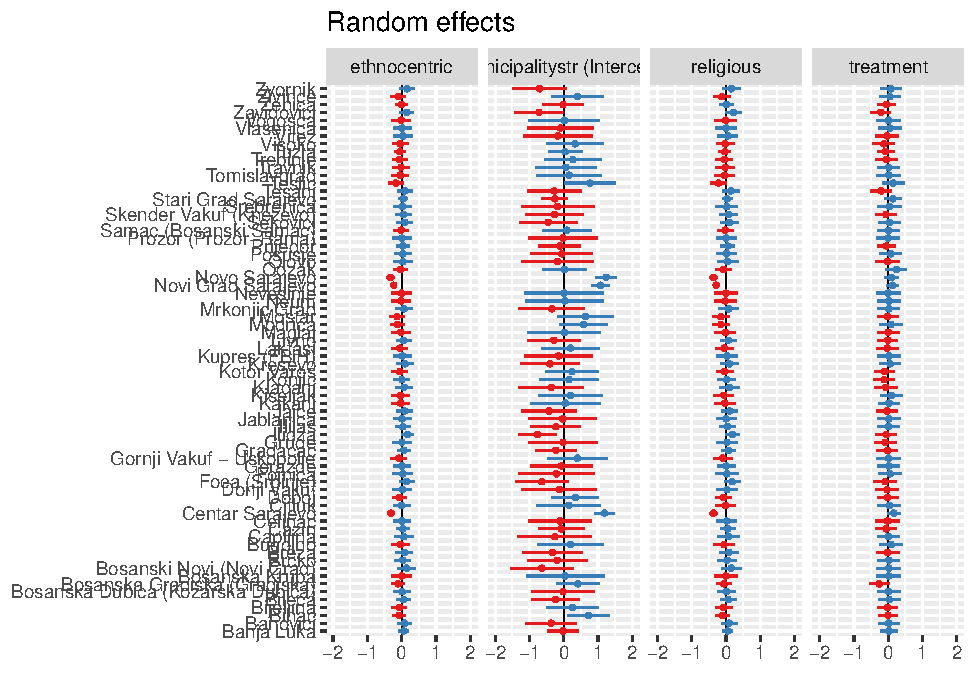
\includegraphics{SMI205_Assessment2_Template_files/figure-latex/outputs-1.pdf}
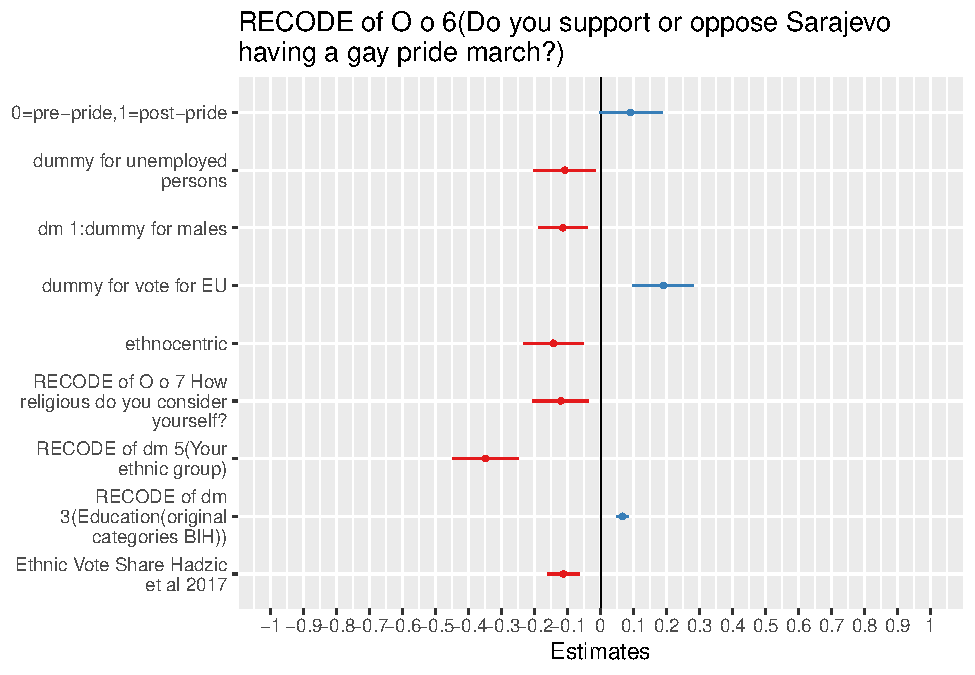
\includegraphics{SMI205_Assessment2_Template_files/figure-latex/outputs-2.pdf}

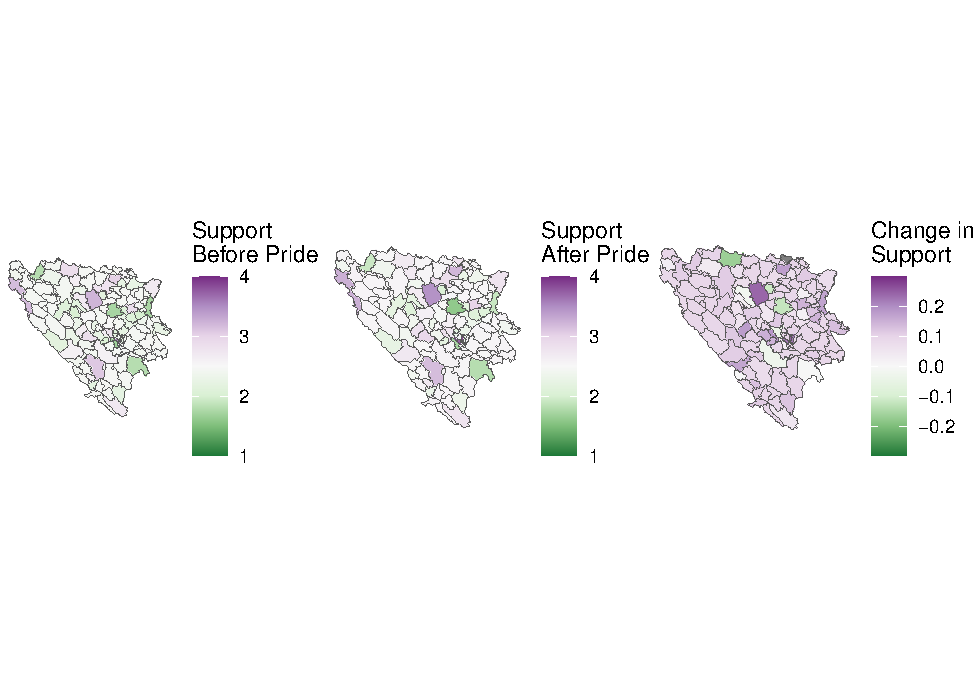
\includegraphics{SMI205_Assessment2_Template_files/figure-latex/maps-1.pdf}

\hypertarget{references}{%
\subsection{References}\label{references}}

Freese, J., \& Peterson, D. (2017). Replication in social science.
\emph{Annual Review of Sociology}, 43, 147-165,
\href{https://www.annualreviews.org/doi/abs/10.1146/annurev-soc-060116-053450}{doi:
10.1146}.

\hypertarget{appendix}{%
\subsection{Appendix}\label{appendix}}

\hypertarget{appendix-1.-my-enviroment-full-information}{%
\subsubsection{Appendix 1. My enviroment (full
information)}\label{appendix-1.-my-enviroment-full-information}}

\begin{Shaded}
\begin{Highlighting}[]
\CommentTok{\# Detailed information about my environment}
\FunctionTok{sessionInfo}\NormalTok{()}
\end{Highlighting}
\end{Shaded}

\begin{verbatim}
R version 4.2.3 (2023-03-15)
Platform: aarch64-apple-darwin20 (64-bit)
Running under: macOS Big Sur 11.7

Matrix products: default
BLAS:   /Library/Frameworks/R.framework/Versions/4.2-arm64/Resources/lib/libRblas.0.dylib
LAPACK: /Library/Frameworks/R.framework/Versions/4.2-arm64/Resources/lib/libRlapack.dylib

locale:
[1] en_US.UTF-8/en_US.UTF-8/en_US.UTF-8/C/en_US.UTF-8/en_US.UTF-8

attached base packages:
[1] stats     graphics  grDevices utils     datasets  methods   base     

other attached packages:
 [1] glmmTMB_1.1.5   sjPlot_2.8.13   lattice_0.20-45 merTools_0.5.2 
 [5] arm_1.13-1      MASS_7.3-58.2   haven_2.5.2     lme4_1.1-31    
 [9] Matrix_1.5-3    ggpubr_0.6.0    geojsonsf_2.0.3 sf_1.0-13      
[13] stringi_1.7.8   lubridate_1.9.2 forcats_1.0.0   stringr_1.5.0  
[17] dplyr_1.1.0     purrr_1.0.1     readr_2.1.4     tidyr_1.3.0    
[21] tibble_3.1.8    ggplot2_3.4.1   tidyverse_2.0.0 knitr_1.41     
[25] rmarkdown_2.18 

loaded via a namespace (and not attached):
 [1] minqa_1.2.5         colorspace_2.0-3    ggsignif_0.6.4     
 [4] ellipsis_0.3.2      class_7.3-21        sjlabelled_1.2.0   
 [7] snakecase_0.11.0    estimability_1.4.1  parameters_0.20.2  
[10] rstudioapi_0.14     proxy_0.4-27        farver_2.1.1       
[13] listenv_0.8.0       furrr_0.3.1         fansi_1.0.3        
[16] mvtnorm_1.1-3       codetools_0.2-19    splines_4.2.3      
[19] sjmisc_2.8.9        nloptr_2.0.3        ggeffects_1.1.5    
[22] broom_1.0.3         broom.mixed_0.2.9.4 effectsize_0.8.3   
[25] shiny_1.7.3         compiler_4.2.3      sjstats_0.18.2     
[28] emmeans_1.8.4-1     backports_1.4.1     fastmap_1.1.0      
[31] cli_3.6.0           later_1.3.0         htmltools_0.5.3    
[34] tools_4.2.3         coda_0.19-4         gtable_0.3.1       
[37] glue_1.6.2          Rcpp_1.0.10         carData_3.0-5      
[40] vctrs_0.5.2         nlme_3.1-162        iterators_1.0.14   
[43] insight_0.19.0      xfun_0.39           globals_0.16.2     
[46] timechange_0.1.1    mime_0.12           lifecycle_1.0.3    
[49] rstatix_0.7.2       future_1.29.0       scales_1.2.1       
[52] hms_1.1.2           promises_1.2.0.1    parallel_4.2.3     
[55] RColorBrewer_1.1-3  TMB_1.9.2           yaml_2.3.6         
[58] highr_0.9           bayestestR_0.13.0   foreach_1.5.2      
[61] e1071_1.7-13        blme_1.0-5          boot_1.3-28.1      
[64] rlang_1.0.6         pkgconfig_2.0.3     evaluate_0.18      
[67] labeling_0.4.2      cowplot_1.1.1       tidyselect_1.2.0   
[70] parallelly_1.32.1   magrittr_2.0.3      R6_2.5.1           
[73] generics_0.1.3      DBI_1.1.3           pillar_1.8.1       
[76] withr_2.5.0         units_0.8-2         datawizard_0.6.5   
[79] abind_1.4-5         performance_0.10.2  modelr_0.1.10      
[82] car_3.1-2           KernSmooth_2.23-20  utf8_1.2.2         
[85] tzdb_0.3.0          grid_4.2.3          digest_0.6.30      
[88] classInt_0.4-9      xtable_1.8-4        httpuv_1.6.6       
[91] numDeriv_2016.8-1.1 munsell_0.5.0      
\end{verbatim}

\hypertarget{appendix-2.-entire-r-code-used-in-the-project}{%
\subsubsection{Appendix 2. Entire R code used in the
project}\label{appendix-2.-entire-r-code-used-in-the-project}}

\begin{Shaded}
\begin{Highlighting}[]
\CommentTok{\# Opening key libraries first}
\FunctionTok{library}\NormalTok{(rmarkdown)}
\FunctionTok{library}\NormalTok{(knitr)}
\CommentTok{\# Global options}
\NormalTok{opts\_chunk}\SpecialCharTok{$}\FunctionTok{set}\NormalTok{(}\AttributeTok{echo=}\ConstantTok{TRUE}\NormalTok{,}
                 \AttributeTok{cache=}\ConstantTok{TRUE}\NormalTok{,}
               \AttributeTok{comment=}\ConstantTok{NA}\NormalTok{,}
               \AttributeTok{message=}\ConstantTok{FALSE}\NormalTok{,}
               \AttributeTok{warning=}\ConstantTok{FALSE}\NormalTok{)}

\CommentTok{\#general}
\FunctionTok{library}\NormalTok{(tidyverse)}

\CommentTok{\#data cleaning}
\FunctionTok{library}\NormalTok{(stringi)}

\CommentTok{\#for maps}
\FunctionTok{library}\NormalTok{(sf)}
\FunctionTok{library}\NormalTok{(geojsonsf)}
\FunctionTok{library}\NormalTok{(ggpubr)}

\CommentTok{\#for modelling}
\FunctionTok{library}\NormalTok{(lme4)}
\FunctionTok{library}\NormalTok{(haven)}
\FunctionTok{library}\NormalTok{(merTools)}
\FunctionTok{library}\NormalTok{(lattice)}

\CommentTok{\#for presenting outputs}
\FunctionTok{library}\NormalTok{(sjPlot)}
\FunctionTok{library}\NormalTok{(glmmTMB)}
\CommentTok{\# Versions of used packages}
\NormalTok{packages }\OtherTok{\textless{}{-}} \FunctionTok{c}\NormalTok{(}\StringTok{"rmarkdown"}\NormalTok{, }\StringTok{"knitr"}\NormalTok{, }\StringTok{"tidyverse"}\NormalTok{, }\StringTok{"stringi"}\NormalTok{, }\StringTok{"sf"}\NormalTok{, }\StringTok{"geojsonsf"}\NormalTok{, }\StringTok{"ggpubr"}\NormalTok{,}
              \StringTok{"lme4"}\NormalTok{, }\StringTok{"haven"}\NormalTok{, }\StringTok{"merTools"}\NormalTok{, }\StringTok{"lattice"}\NormalTok{, }\StringTok{"sjPlot"}\NormalTok{, }\StringTok{"glmmTMB"}\NormalTok{)}
\FunctionTok{names}\NormalTok{(packages) }\OtherTok{\textless{}{-}}\NormalTok{ packages}
\FunctionTok{lapply}\NormalTok{(packages, packageVersion)}
\CommentTok{\# What is my R version?}
\NormalTok{version[[}\StringTok{\textquotesingle{}version.string\textquotesingle{}}\NormalTok{]]}
\CommentTok{\#Data}
\CommentTok{\#Read data and shapefile}
\NormalTok{rep\_data }\OtherTok{\textless{}{-}} \FunctionTok{read\_dta}\NormalTok{(}\StringTok{\textquotesingle{}Data/Pride\_Amid\_Prejudice\_replication data\_final.dta\textquotesingle{}}\NormalTok{)}
\NormalTok{shape }\OtherTok{\textless{}{-}} \FunctionTok{geojson\_sf}\NormalTok{(}\StringTok{"Data/geoBoundaries{-}BIH{-}ADM2.geojson"}\NormalTok{)}

\CommentTok{\#Remove non{-}Latin characters and macth name discrepencies, eg.}
\NormalTok{shape}\SpecialCharTok{$}\NormalTok{shapeName }\OtherTok{=} \FunctionTok{stri\_trans\_general}\NormalTok{(}\AttributeTok{str =}\NormalTok{ shape}\SpecialCharTok{$}\NormalTok{shapeName, }\AttributeTok{id =} \StringTok{"Latin{-}ASCII"}\NormalTok{)}
\NormalTok{shape[}\DecValTok{15}\NormalTok{, }\StringTok{"shapeName"}\NormalTok{] }\OtherTok{\textless{}{-}} \StringTok{"Bosanska Gradiska (Gradiska)"}
\NormalTok{shape[}\DecValTok{18}\NormalTok{, }\StringTok{"shapeName"}\NormalTok{] }\OtherTok{\textless{}{-}} \StringTok{"Bosanska Dubica (Kozarska Dubica)"}
\NormalTok{shape[}\DecValTok{20}\NormalTok{, }\StringTok{"shapeName"}\NormalTok{] }\OtherTok{\textless{}{-}} \StringTok{"Bosanski Novi (Novi Grad)"}
\NormalTok{shape[}\DecValTok{22}\NormalTok{, }\StringTok{"shapeName"}\NormalTok{] }\OtherTok{\textless{}{-}} \StringTok{"Samac (Bosanski Samac)"}
\NormalTok{shape[}\DecValTok{23}\NormalTok{, }\StringTok{"shapeName"}\NormalTok{] }\OtherTok{\textless{}{-}} \StringTok{"Bosansko Grahovo (Grahovo)"}
\NormalTok{shape[}\DecValTok{1}\NormalTok{, }\StringTok{"shapeName"}\NormalTok{] }\OtherTok{\textless{}{-}} \StringTok{"Brcko"}
\NormalTok{shape[}\DecValTok{33}\NormalTok{, }\StringTok{"shapeName"}\NormalTok{] }\OtherTok{\textless{}{-}} \StringTok{"Centar Sarajevo"}
\NormalTok{shape[}\DecValTok{48}\NormalTok{, }\StringTok{"shapeName"}\NormalTok{] }\OtherTok{\textless{}{-}} \StringTok{"Foca (Srbinje)"}
\NormalTok{shape[}\DecValTok{53}\NormalTok{, }\StringTok{"shapeName"}\NormalTok{] }\OtherTok{\textless{}{-}} \StringTok{"Gornji Vakuf {-} Uskopolje"}
\NormalTok{shape[}\DecValTok{74}\NormalTok{, }\StringTok{"shapeName"}\NormalTok{] }\OtherTok{\textless{}{-}} \StringTok{"Kupres (FBiH)"}
\NormalTok{shape[}\DecValTok{89}\NormalTok{, }\StringTok{"shapeName"}\NormalTok{] }\OtherTok{\textless{}{-}} \StringTok{"Novi Grad Sarajevo"}
\NormalTok{shape[}\DecValTok{97}\NormalTok{, }\StringTok{"shapeName"}\NormalTok{] }\OtherTok{\textless{}{-}} \StringTok{"Pale (RS)"}
\NormalTok{shape[}\DecValTok{104}\NormalTok{, }\StringTok{"shapeName"}\NormalTok{] }\OtherTok{\textless{}{-}} \StringTok{"Prozor (Prozor{-}Rama)"}
\NormalTok{shape[}\DecValTok{114}\NormalTok{, }\StringTok{"shapeName"}\NormalTok{] }\OtherTok{\textless{}{-}} \StringTok{"Skender Vakuf (Knezevo)"}
\NormalTok{shape[}\DecValTok{92}\NormalTok{, }\StringTok{"shapeName"}\NormalTok{] }\OtherTok{\textless{}{-}} \StringTok{"Stari Grad Sarajevo"}
\NormalTok{shape[}\DecValTok{125}\NormalTok{, }\StringTok{"shapeName"}\NormalTok{] }\OtherTok{\textless{}{-}} \StringTok{"Trnovo (FBiH)"}
\NormalTok{shape[}\DecValTok{139}\NormalTok{, }\StringTok{"shapeName"}\NormalTok{] }\OtherTok{\textless{}{-}} \StringTok{"Zivince"}
\CommentTok{\#Merge survey data and shapefile}
\NormalTok{rep\_shape }\OtherTok{\textless{}{-}} \FunctionTok{inner\_join}\NormalTok{(rep\_data, shape, }\AttributeTok{by =} \FunctionTok{join\_by}\NormalTok{(}\StringTok{"municipalitystr"} \SpecialCharTok{==} \StringTok{"shapeName"}\NormalTok{))}
\CommentTok{\#Remove observations with missing data}
\NormalTok{rep\_shape\_m }\OtherTok{\textless{}{-}}\NormalTok{ rep\_shape[}\FunctionTok{complete.cases}\NormalTok{(rep\_shape[,}\FunctionTok{c}\NormalTok{(}\StringTok{\textquotesingle{}ethnocentric\textquotesingle{}}\NormalTok{, }\StringTok{\textquotesingle{}religious\textquotesingle{}}\NormalTok{, }\StringTok{\textquotesingle{}Education\textquotesingle{}}\NormalTok{)]),]}
\CommentTok{\#Rescale variables}
\NormalTok{rep\_shape\_m}\SpecialCharTok{$}\NormalTok{vote\_share\_10 }\OtherTok{\textless{}{-}}\NormalTok{ rep\_shape\_m}\SpecialCharTok{$}\NormalTok{ethnic\_vote\_share}\SpecialCharTok{/}\DecValTok{10}
\NormalTok{rep\_shape\_m}\SpecialCharTok{$}\NormalTok{age\_10 }\OtherTok{\textless{}{-}}\NormalTok{ rep\_shape\_m}\SpecialCharTok{$}\NormalTok{age}\SpecialCharTok{/}\DecValTok{10}
\DocumentationTok{\#\#\#Distribution of Respondents}
\CommentTok{\#count respondents by municipality}
\NormalTok{resp\_muni }\OtherTok{\textless{}{-}} \FunctionTok{as.data.frame}\NormalTok{(}\FunctionTok{table}\NormalTok{(rep\_data}\SpecialCharTok{$}\NormalTok{municipalitystr))}
\CommentTok{\#merge }
\NormalTok{resp\_muni\_shape }\OtherTok{\textless{}{-}} \FunctionTok{full\_join}\NormalTok{(resp\_muni, shape, }\AttributeTok{by =} \FunctionTok{join\_by}\NormalTok{(}\StringTok{"Var1"} \SpecialCharTok{==} \StringTok{"shapeName"}\NormalTok{))}
\CommentTok{\#remove the blank municipality value, turn NAs to 0}
\NormalTok{resp\_muni\_shape }\OtherTok{\textless{}{-}}\NormalTok{ resp\_muni\_shape[}\SpecialCharTok{{-}}\NormalTok{(}\DecValTok{1}\NormalTok{),]}
\NormalTok{resp\_muni\_shape}\SpecialCharTok{$}\NormalTok{Freq }\OtherTok{\textless{}{-}}\NormalTok{ resp\_muni\_shape}\SpecialCharTok{$}\NormalTok{Freq }\SpecialCharTok{\%\textgreater{}\%} \FunctionTok{replace}\NormalTok{(}\FunctionTok{is.na}\NormalTok{(.),}\DecValTok{0}\NormalTok{)}
\CommentTok{\#histogram of number of respondents by municipality}
\FunctionTok{ggplot}\NormalTok{(resp\_muni\_shape) }\SpecialCharTok{+}
  \FunctionTok{aes}\NormalTok{(}\AttributeTok{x =}\NormalTok{ Freq) }\SpecialCharTok{+}
  \FunctionTok{geom\_histogram}\NormalTok{(}\AttributeTok{binwidth =} \DecValTok{10}\NormalTok{)}

\CommentTok{\#map of number of respondents by municipality}
\FunctionTok{ggplot}\NormalTok{(resp\_muni\_shape) }\SpecialCharTok{+}
  \FunctionTok{aes}\NormalTok{(}\AttributeTok{geometry =}\NormalTok{ geometry, }\AttributeTok{fill =} \FunctionTok{cut}\NormalTok{(Freq,}
                                      \AttributeTok{breaks =} \FunctionTok{c}\NormalTok{(}\SpecialCharTok{{-}}\DecValTok{1}\NormalTok{,}\DecValTok{0}\NormalTok{,}\DecValTok{10}\NormalTok{,}\DecValTok{20}\NormalTok{,}\DecValTok{30}\NormalTok{,}\DecValTok{40}\NormalTok{,}\DecValTok{50}\NormalTok{,}\DecValTok{320}\NormalTok{))) }\SpecialCharTok{+}
  \FunctionTok{geom\_sf}\NormalTok{() }\SpecialCharTok{+}
  \FunctionTok{scale\_fill\_grey}\NormalTok{(}\AttributeTok{start =} \DecValTok{1}\NormalTok{, }\AttributeTok{end =} \FloatTok{0.1}\NormalTok{) }\SpecialCharTok{+}
  \FunctionTok{labs}\NormalTok{(}\AttributeTok{fill =} \StringTok{"respondents"}\NormalTok{) }\SpecialCharTok{+} \FunctionTok{theme\_void}\NormalTok{()}
\DocumentationTok{\#\#\#null model}
\CommentTok{\#need to figure out which data to use to make the plot work}
\NormalTok{null.m }\OtherTok{\textless{}{-}} \FunctionTok{lmer}\NormalTok{(supportpride }\SpecialCharTok{\textasciitilde{}}\NormalTok{ (}\DecValTok{1}\SpecialCharTok{|}\NormalTok{municipalitystr), }\AttributeTok{data =}\NormalTok{ rep\_shape\_m, }\AttributeTok{na.action=}\StringTok{"na.exclude"}\NormalTok{)}
\FunctionTok{summary}\NormalTok{(null.m)}
\NormalTok{pred.null.m }\OtherTok{\textless{}{-}} \FunctionTok{fitted}\NormalTok{(null.m)}

\FunctionTok{ggplot}\NormalTok{(rep\_shape\_m) }\SpecialCharTok{+}
  \FunctionTok{aes}\NormalTok{(}\AttributeTok{x=}\NormalTok{treatment, }\AttributeTok{y =}\NormalTok{ pred.null.m, }\AttributeTok{group =}\NormalTok{ municipalitystr) }\SpecialCharTok{+}
  \FunctionTok{geom\_line}\NormalTok{() }\SpecialCharTok{+}
  \FunctionTok{scale\_color\_continuous}\NormalTok{(}\AttributeTok{guide =} \StringTok{\textquotesingle{}none\textquotesingle{}}\NormalTok{) }

\NormalTok{VPC }\OtherTok{=} \FloatTok{0.1036}\SpecialCharTok{/}\NormalTok{(}\FloatTok{0.1036+0.8145}\NormalTok{)}
\CommentTok{\#=11.3\% variation explained by municipality. more variation at individual level}
\DocumentationTok{\#\#\#random slopes models}
\NormalTok{slopes.m }\OtherTok{\textless{}{-}} \FunctionTok{lmer}\NormalTok{(supportpride }\SpecialCharTok{\textasciitilde{}}\NormalTok{ treatment }\SpecialCharTok{+}\NormalTok{ (}\DecValTok{1} \SpecialCharTok{+}\NormalTok{ treatment}\SpecialCharTok{|}\NormalTok{municipalitystr), }\AttributeTok{data =}\NormalTok{ rep\_shape\_m, }\AttributeTok{na.action=}\StringTok{"na.exclude"}\NormalTok{)}
\FunctionTok{summary}\NormalTok{(slopes.m)}

\NormalTok{pred.slopes.m }\OtherTok{\textless{}{-}} \FunctionTok{fitted}\NormalTok{(slopes.m)}

\FunctionTok{ggplot}\NormalTok{(rep\_shape\_m) }\SpecialCharTok{+}
  \FunctionTok{aes}\NormalTok{(}\AttributeTok{x=}\NormalTok{treatment, }\AttributeTok{y =}\NormalTok{ pred.slopes.m, }\AttributeTok{group =}\NormalTok{ municipalitystr) }\SpecialCharTok{+}
  \FunctionTok{geom\_line}\NormalTok{() }\SpecialCharTok{+}
  \FunctionTok{scale\_color\_continuous}\NormalTok{(}\AttributeTok{guide =} \StringTok{\textquotesingle{}none\textquotesingle{}}\NormalTok{) }
\CommentTok{\#plot shows fanning out: most supportive become more supportive; least become less}
\CommentTok{\#add highlight to this to show sarajevo municipalities}

\NormalTok{u.slopes.m }\OtherTok{\textless{}{-}} \FunctionTok{ranef}\NormalTok{(slopes.m, }\AttributeTok{condVar =}\NormalTok{ T)}
\FunctionTok{dotplot}\NormalTok{(u.slopes.m)}

\NormalTok{reEX.slopes.m }\OtherTok{\textless{}{-}}  \FunctionTok{REsim}\NormalTok{(slopes.m)}
\FunctionTok{plotREsim}\NormalTok{(reEX.slopes.m, }\AttributeTok{labs =}\NormalTok{ T)}

\DocumentationTok{\#\#\#\#gender{-}{-}{-}{-}}
\NormalTok{slopes}\FloatTok{.1}\NormalTok{a }\OtherTok{\textless{}{-}} \FunctionTok{lmer}\NormalTok{(supportpride }\SpecialCharTok{\textasciitilde{}}\NormalTok{ treatment }\SpecialCharTok{+}\NormalTok{ Men }\SpecialCharTok{+}\NormalTok{ (}\DecValTok{1} \SpecialCharTok{+}\NormalTok{ treatment}\SpecialCharTok{|}\NormalTok{municipalitystr),}
                  \AttributeTok{data =}\NormalTok{ rep\_shape\_m, }\AttributeTok{na.action=}\StringTok{"na.exclude"}\NormalTok{)}

\NormalTok{slopes}\FloatTok{.1}\NormalTok{b }\OtherTok{\textless{}{-}} \FunctionTok{lmer}\NormalTok{(supportpride }\SpecialCharTok{\textasciitilde{}}\NormalTok{ treatment }\SpecialCharTok{+}\NormalTok{ Men }\SpecialCharTok{+}\NormalTok{ (}\DecValTok{1} \SpecialCharTok{+}\NormalTok{ treatment }\SpecialCharTok{+}\NormalTok{ Men }\SpecialCharTok{|}\NormalTok{ municipalitystr),}
                  \AttributeTok{data =}\NormalTok{ rep\_shape\_m, }\AttributeTok{na.action=}\StringTok{"na.exclude"}\NormalTok{)}

\FunctionTok{anova}\NormalTok{(slopes}\FloatTok{.1}\NormalTok{a, slopes}\FloatTok{.1}\NormalTok{b)}
\CommentTok{\#AIC and Chi show no significant evidence of the effect of gender varying by municipality, }
\CommentTok{\#slope.1a better fit}

\DocumentationTok{\#\#\#\#unemployed{-}{-}{-}{-}}
\NormalTok{slopes}\FloatTok{.2}\NormalTok{a }\OtherTok{\textless{}{-}} \FunctionTok{lmer}\NormalTok{(supportpride }\SpecialCharTok{\textasciitilde{}}\NormalTok{ treatment }\SpecialCharTok{+}\NormalTok{ unemployed }\SpecialCharTok{+}\NormalTok{ Men }\SpecialCharTok{+}\NormalTok{ (}\DecValTok{1} \SpecialCharTok{+}\NormalTok{ treatment}\SpecialCharTok{|}\NormalTok{municipalitystr),}
                  \AttributeTok{data =}\NormalTok{ rep\_shape\_m, }\AttributeTok{na.action=}\StringTok{"na.exclude"}\NormalTok{)}

\FunctionTok{anova}\NormalTok{(slopes}\FloatTok{.2}\NormalTok{a, slopes}\FloatTok{.1}\NormalTok{a) }\CommentTok{\#better than 1a}

\DocumentationTok{\#\#\#\#voteeu{-}{-}{-}{-}}
\NormalTok{(slopes}\FloatTok{.3}\NormalTok{a }\OtherTok{\textless{}{-}} \FunctionTok{lmer}\NormalTok{(supportpride }\SpecialCharTok{\textasciitilde{}}\NormalTok{ treatment }\SpecialCharTok{+}\NormalTok{ unemployed }\SpecialCharTok{+}\NormalTok{ Men }\SpecialCharTok{+}\NormalTok{ voteeu }\SpecialCharTok{+}\NormalTok{ (}\DecValTok{1} \SpecialCharTok{+}\NormalTok{ treatment}\SpecialCharTok{|}\NormalTok{municipalitystr),}
                   \AttributeTok{data =}\NormalTok{ rep\_shape\_m, }\AttributeTok{na.action=}\StringTok{"na.exclude"}\NormalTok{))}

\NormalTok{(slopes}\FloatTok{.3}\NormalTok{b }\OtherTok{\textless{}{-}} \FunctionTok{lmer}\NormalTok{(supportpride }\SpecialCharTok{\textasciitilde{}}\NormalTok{ treatment }\SpecialCharTok{+}\NormalTok{ unemployed }\SpecialCharTok{+}\NormalTok{ Men }\SpecialCharTok{+}\NormalTok{ voteeu }\SpecialCharTok{+}\NormalTok{ (}\DecValTok{1} \SpecialCharTok{+}\NormalTok{ treatment }\SpecialCharTok{+}\NormalTok{ voteeu}\SpecialCharTok{|}\NormalTok{municipalitystr),}
                   \AttributeTok{data =}\NormalTok{ rep\_shape\_m, }\AttributeTok{na.action=}\StringTok{"na.exclude"}\NormalTok{))}

\FunctionTok{anova}\NormalTok{(slopes}\FloatTok{.3}\NormalTok{a, slopes}\FloatTok{.3}\NormalTok{b) }\CommentTok{\#3a better}
\CommentTok{\#Example of testing for random effects}
\NormalTok{(slopes}\FloatTok{.4}\NormalTok{a }\OtherTok{\textless{}{-}} \FunctionTok{lmer}\NormalTok{(supportpride }\SpecialCharTok{\textasciitilde{}}\NormalTok{ treatment }\SpecialCharTok{+}\NormalTok{ unemployed }\SpecialCharTok{+}\NormalTok{ Men }\SpecialCharTok{+}\NormalTok{ voteeu }\SpecialCharTok{+}\NormalTok{ ethnocentric }\SpecialCharTok{+}\NormalTok{ (}\DecValTok{1} \SpecialCharTok{+}\NormalTok{ treatment}\SpecialCharTok{|}\NormalTok{municipalitystr),}
                   \AttributeTok{data =}\NormalTok{ rep\_shape\_m, }\AttributeTok{na.action=}\StringTok{"na.exclude"}\NormalTok{))}

\NormalTok{(slopes}\FloatTok{.4}\NormalTok{b }\OtherTok{\textless{}{-}} \FunctionTok{lmer}\NormalTok{(supportpride }\SpecialCharTok{\textasciitilde{}}\NormalTok{ treatment }\SpecialCharTok{+}\NormalTok{ unemployed }\SpecialCharTok{+}\NormalTok{ Men }\SpecialCharTok{+}\NormalTok{ voteeu }\SpecialCharTok{+}\NormalTok{ ethnocentric }\SpecialCharTok{+}\NormalTok{ (}\DecValTok{1} \SpecialCharTok{+}\NormalTok{ treatment }\SpecialCharTok{+}\NormalTok{ ethnocentric}\SpecialCharTok{|}\NormalTok{municipalitystr),}
                   \AttributeTok{data =}\NormalTok{ rep\_shape\_m, }\AttributeTok{na.action=}\StringTok{"na.exclude"}\NormalTok{))}

\FunctionTok{anova}\NormalTok{(slopes}\FloatTok{.4}\NormalTok{b, slopes}\FloatTok{.4}\NormalTok{a) }\CommentTok{\#4b better, effect of ethnocentrism varies by municipality}
\FunctionTok{summary}\NormalTok{(slopes}\FloatTok{.4}\NormalTok{b) }\CommentTok{\#is the effect significant?}
\FunctionTok{anova}\NormalTok{(slopes}\FloatTok{.3}\NormalTok{a, slopes}\FloatTok{.4}\NormalTok{b) }\CommentTok{\#better than the earlier model}

\DocumentationTok{\#\#\#\#religiosity{-}{-}{-}{-}}
\NormalTok{(slopes}\FloatTok{.5}\NormalTok{a }\OtherTok{\textless{}{-}} \FunctionTok{lmer}\NormalTok{(supportpride }\SpecialCharTok{\textasciitilde{}}\NormalTok{ treatment }\SpecialCharTok{+}\NormalTok{ unemployed }\SpecialCharTok{+}\NormalTok{ Men }\SpecialCharTok{+}\NormalTok{ voteeu }\SpecialCharTok{+}\NormalTok{ ethnocentric }\SpecialCharTok{+}\NormalTok{ religious }\SpecialCharTok{+}\NormalTok{ (}\DecValTok{1} \SpecialCharTok{+}\NormalTok{ treatment }\SpecialCharTok{+}\NormalTok{ ethnocentric}\SpecialCharTok{|}\NormalTok{municipalitystr),}
                   \AttributeTok{data =}\NormalTok{ rep\_shape\_m, }\AttributeTok{na.action=}\StringTok{"na.exclude"}\NormalTok{))}

\NormalTok{(slopes}\FloatTok{.5}\NormalTok{b }\OtherTok{\textless{}{-}} \FunctionTok{lmer}\NormalTok{(supportpride }\SpecialCharTok{\textasciitilde{}}\NormalTok{ treatment }\SpecialCharTok{+}\NormalTok{ unemployed }\SpecialCharTok{+}\NormalTok{ Men }\SpecialCharTok{+}\NormalTok{ voteeu }\SpecialCharTok{+}\NormalTok{ ethnocentric }\SpecialCharTok{+}\NormalTok{ religious }\SpecialCharTok{+}\NormalTok{ (}\DecValTok{1} \SpecialCharTok{+}\NormalTok{ treatment }\SpecialCharTok{+}\NormalTok{ ethnocentric }\SpecialCharTok{+}\NormalTok{ religious}\SpecialCharTok{|}\NormalTok{municipalitystr),}
                   \AttributeTok{data =}\NormalTok{ rep\_shape\_m, }\AttributeTok{na.action=}\StringTok{"na.exclude"}\NormalTok{))}

\FunctionTok{anova}\NormalTok{(slopes}\FloatTok{.5}\NormalTok{a, slopes}\FloatTok{.5}\NormalTok{b) }

\DocumentationTok{\#\#\#\#Bosniak, Croat, Serb; Bosnian as reference{-}{-}{-}{-}}
\NormalTok{(slopes}\FloatTok{.6}\NormalTok{a }\OtherTok{\textless{}{-}} \FunctionTok{lmer}\NormalTok{(supportpride }\SpecialCharTok{\textasciitilde{}}\NormalTok{ treatment }\SpecialCharTok{+}\NormalTok{ unemployed }\SpecialCharTok{+}\NormalTok{ Men }\SpecialCharTok{+}\NormalTok{ voteeu }\SpecialCharTok{+}\NormalTok{ ethnocentric }\SpecialCharTok{+}\NormalTok{ religious }\SpecialCharTok{+} 
\NormalTok{                     Bosniak }\SpecialCharTok{+}\NormalTok{ Croat }\SpecialCharTok{+}\NormalTok{ Serb }\SpecialCharTok{+}\NormalTok{ (}\DecValTok{1} \SpecialCharTok{+}\NormalTok{ treatment }\SpecialCharTok{+}\NormalTok{ ethnocentric }\SpecialCharTok{+}\NormalTok{ religious}\SpecialCharTok{|}\NormalTok{municipalitystr),}
                   \AttributeTok{data =}\NormalTok{ rep\_shape\_m, }\AttributeTok{na.action=}\StringTok{"na.exclude"}\NormalTok{))}

\NormalTok{(slopes}\FloatTok{.6}\NormalTok{b }\OtherTok{\textless{}{-}} \FunctionTok{lmer}\NormalTok{(supportpride }\SpecialCharTok{\textasciitilde{}}\NormalTok{ treatment }\SpecialCharTok{+}\NormalTok{ unemployed }\SpecialCharTok{+}\NormalTok{ Men }\SpecialCharTok{+}\NormalTok{ voteeu }\SpecialCharTok{+}\NormalTok{ ethnocentric }\SpecialCharTok{+}\NormalTok{ religious }\SpecialCharTok{+} 
\NormalTok{                     Bosniak }\SpecialCharTok{+}\NormalTok{ Croat }\SpecialCharTok{+}\NormalTok{ Serb }\SpecialCharTok{+}\NormalTok{ (}\DecValTok{1} \SpecialCharTok{+}\NormalTok{ treatment }\SpecialCharTok{+}\NormalTok{ ethnocentric }\SpecialCharTok{+}\NormalTok{ religious }\SpecialCharTok{+}\NormalTok{ Bosniak }\SpecialCharTok{+}\NormalTok{ Serb }\SpecialCharTok{+}\NormalTok{ Croat}\SpecialCharTok{|}\NormalTok{municipalitystr),}
                   \AttributeTok{data =}\NormalTok{ rep\_shape\_m, }\AttributeTok{na.action=}\StringTok{"na.exclude"}\NormalTok{))}
\FunctionTok{anova}\NormalTok{(slopes}\FloatTok{.6}\NormalTok{a, slopes}\FloatTok{.6}\NormalTok{b) }\CommentTok{\#not significantly better, use 6a}
\FunctionTok{summary}\NormalTok{(slopes}\FloatTok{.6}\NormalTok{a) }\CommentTok{\#Croat not significant, omit from further models}

\DocumentationTok{\#\#\#\#education{-}{-}{-}{-}}
\NormalTok{(slopes}\FloatTok{.7}\NormalTok{a }\OtherTok{\textless{}{-}} \FunctionTok{lmer}\NormalTok{(supportpride }\SpecialCharTok{\textasciitilde{}}\NormalTok{ treatment }\SpecialCharTok{+}\NormalTok{ unemployed }\SpecialCharTok{+}\NormalTok{ Men }\SpecialCharTok{+}\NormalTok{ voteeu }\SpecialCharTok{+}\NormalTok{ ethnocentric }\SpecialCharTok{+}\NormalTok{ religious }\SpecialCharTok{+} 
\NormalTok{                     Bosniak }\SpecialCharTok{+}\NormalTok{ Serb }\SpecialCharTok{+}\NormalTok{ Education }\SpecialCharTok{+}\NormalTok{ (}\DecValTok{1} \SpecialCharTok{+}\NormalTok{ treatment }\SpecialCharTok{+}\NormalTok{ ethnocentric }\SpecialCharTok{+}\NormalTok{ religious}\SpecialCharTok{|}\NormalTok{municipalitystr),}
                   \AttributeTok{data =}\NormalTok{ rep\_shape\_m, }\AttributeTok{na.action=}\StringTok{"na.exclude"}\NormalTok{))}



\DocumentationTok{\#\#\#\#ethnic vote share{-}{-}{-}{-}}
\NormalTok{(slopes}\FloatTok{.8}\NormalTok{a }\OtherTok{\textless{}{-}} \FunctionTok{lmer}\NormalTok{(supportpride }\SpecialCharTok{\textasciitilde{}}\NormalTok{ treatment }\SpecialCharTok{+}\NormalTok{ unemployed }\SpecialCharTok{+}\NormalTok{ Men }\SpecialCharTok{+}\NormalTok{ voteeu }\SpecialCharTok{+}\NormalTok{ ethnocentric }\SpecialCharTok{+}\NormalTok{ religious }\SpecialCharTok{+} 
\NormalTok{                     Bosniak }\SpecialCharTok{+}\NormalTok{ Serb }\SpecialCharTok{+}\NormalTok{ Education }\SpecialCharTok{+}\NormalTok{ vote\_share\_10 }\SpecialCharTok{+}\NormalTok{ (}\DecValTok{1} \SpecialCharTok{+}\NormalTok{ treatment }\SpecialCharTok{+}\NormalTok{ ethnocentric }\SpecialCharTok{+}\NormalTok{ religious}\SpecialCharTok{|}\NormalTok{municipalitystr),}
                   \AttributeTok{data =}\NormalTok{ rep\_shape\_m, }\AttributeTok{na.action=}\StringTok{"na.exclude"}\NormalTok{))}

\FunctionTok{summary}\NormalTok{(slopes}\FloatTok{.8}\NormalTok{a)}
\CommentTok{\#when account for vote share, serb no longer significant}
\FunctionTok{cor.test}\NormalTok{(rep\_shape\_m}\SpecialCharTok{$}\NormalTok{vote\_share\_10, rep\_shape\_m}\SpecialCharTok{$}\NormalTok{Serb) }\CommentTok{\#strong correlation between vote share and serb}
\CommentTok{\#remove serb from now on}

\DocumentationTok{\#\#\#\#age{-}{-}{-}{-}}
\NormalTok{(slopes}\FloatTok{.9}\NormalTok{a }\OtherTok{\textless{}{-}} \FunctionTok{lmer}\NormalTok{(supportpride }\SpecialCharTok{\textasciitilde{}}\NormalTok{ treatment }\SpecialCharTok{+}\NormalTok{ unemployed }\SpecialCharTok{+}\NormalTok{ Men }\SpecialCharTok{+}\NormalTok{ voteeu }\SpecialCharTok{+}\NormalTok{ ethnocentric }\SpecialCharTok{+}\NormalTok{ religious }\SpecialCharTok{+} 
\NormalTok{                     Bosniak }\SpecialCharTok{+}\NormalTok{ Education }\SpecialCharTok{+}\NormalTok{ vote\_share\_10 }\SpecialCharTok{+}\NormalTok{ age\_10 }\SpecialCharTok{+}\NormalTok{ (}\DecValTok{1} \SpecialCharTok{+}\NormalTok{ treatment }\SpecialCharTok{+}\NormalTok{ ethnocentric }\SpecialCharTok{+}\NormalTok{ religious}\SpecialCharTok{|}\NormalTok{municipalitystr),}
                   \AttributeTok{data =}\NormalTok{ rep\_shape\_m, }\AttributeTok{na.action=}\StringTok{"na.exclude"}\NormalTok{))}
\FunctionTok{summary}\NormalTok{(slopes}\FloatTok{.9}\NormalTok{a) }\CommentTok{\#age not significant, remove from future models}

\DocumentationTok{\#\#\#\#casualty{-}{-}{-}{-}}
\NormalTok{(slopes}\FloatTok{.10}\NormalTok{a }\OtherTok{\textless{}{-}} \FunctionTok{lmer}\NormalTok{(supportpride }\SpecialCharTok{\textasciitilde{}}\NormalTok{ treatment }\SpecialCharTok{+}\NormalTok{ unemployed }\SpecialCharTok{+}\NormalTok{ Men }\SpecialCharTok{+}\NormalTok{ voteeu }\SpecialCharTok{+}\NormalTok{ ethnocentric }\SpecialCharTok{+}\NormalTok{ religious }\SpecialCharTok{+} 
\NormalTok{                      Bosniak }\SpecialCharTok{+}\NormalTok{ Education }\SpecialCharTok{+}\NormalTok{ vote\_share\_10 }\SpecialCharTok{+}\NormalTok{ casualty }\SpecialCharTok{+}\NormalTok{ (}\DecValTok{1} \SpecialCharTok{+}\NormalTok{ treatment }\SpecialCharTok{+}\NormalTok{ ethnocentric }\SpecialCharTok{+}\NormalTok{ religious}\SpecialCharTok{|}\NormalTok{municipalitystr),}
                    \AttributeTok{data =}\NormalTok{ rep\_shape\_m, }\AttributeTok{na.action=}\StringTok{"na.exclude"}\NormalTok{))}
\FunctionTok{summary}\NormalTok{(slopes}\FloatTok{.10}\NormalTok{a) }\CommentTok{\#casualty not significant}

\DocumentationTok{\#\#\#\#population density{-}{-}{-}{-}}
\NormalTok{slopes}\FloatTok{.11}\NormalTok{a }\OtherTok{\textless{}{-}} \FunctionTok{lmer}\NormalTok{(supportpride }\SpecialCharTok{\textasciitilde{}}\NormalTok{ treatment }\SpecialCharTok{+}\NormalTok{ unemployed }\SpecialCharTok{+}\NormalTok{ Men }\SpecialCharTok{+}\NormalTok{ voteeu }\SpecialCharTok{+}\NormalTok{ ethnocentric }\SpecialCharTok{+}\NormalTok{ religious }\SpecialCharTok{+} 
\NormalTok{                     Bosniak }\SpecialCharTok{+}\NormalTok{ Education }\SpecialCharTok{+}\NormalTok{ vote\_share\_10 }\SpecialCharTok{+}\NormalTok{ log\_pop\_density }\SpecialCharTok{+}
\NormalTok{                     (}\DecValTok{1} \SpecialCharTok{+}\NormalTok{ treatment }\SpecialCharTok{+}\NormalTok{ ethnocentric }\SpecialCharTok{+}\NormalTok{ religious}\SpecialCharTok{|}\NormalTok{municipalitystr),}
                   \AttributeTok{data =}\NormalTok{ rep\_shape\_m, }\AttributeTok{na.action=}\StringTok{"na.exclude"}\NormalTok{)}
\FunctionTok{summary}\NormalTok{(slopes}\FloatTok{.11}\NormalTok{a) }\CommentTok{\#not significant }
\NormalTok{slopes.final }\OtherTok{\textless{}{-}} \FunctionTok{lmer}\NormalTok{(supportpride }\SpecialCharTok{\textasciitilde{}}\NormalTok{ treatment }\SpecialCharTok{+}\NormalTok{ unemployed }\SpecialCharTok{+}\NormalTok{ Men }\SpecialCharTok{+}\NormalTok{ voteeu }\SpecialCharTok{+}\NormalTok{ ethnocentric }\SpecialCharTok{+} 
\NormalTok{                       religious }\SpecialCharTok{+}\NormalTok{ Bosniak }\SpecialCharTok{+}\NormalTok{ Education }\SpecialCharTok{+}\NormalTok{ vote\_share\_10 }\SpecialCharTok{+} 
\NormalTok{                        (}\DecValTok{1} \SpecialCharTok{+}\NormalTok{ treatment }\SpecialCharTok{+}\NormalTok{ ethnocentric }\SpecialCharTok{+}\NormalTok{ religious}\SpecialCharTok{|}\NormalTok{municipalitystr),}
                           \AttributeTok{data =}\NormalTok{ rep\_shape\_m, }\AttributeTok{na.action=}\StringTok{"na.exclude"}\NormalTok{)}
\DocumentationTok{\#\#Results{-}{-}{-}{-}}

\DocumentationTok{\#\#\#}
\NormalTok{pred.slopes.final }\OtherTok{\textless{}{-}} \FunctionTok{fitted}\NormalTok{(slopes.final)}
\NormalTok{rep\_shape\_m}\SpecialCharTok{$}\NormalTok{pred.slopes.final }\OtherTok{\textless{}{-}}\NormalTok{ pred.slopes.final}
\NormalTok{rep\_shape\_p }\OtherTok{\textless{}{-}} \FunctionTok{full\_join}\NormalTok{(rep\_shape\_m, shape, }\AttributeTok{by =} \FunctionTok{join\_by}\NormalTok{(}\StringTok{"municipalitystr"} \SpecialCharTok{==} \StringTok{"shapeName"}\NormalTok{))}
\NormalTok{rep\_shape\_p }\OtherTok{\textless{}{-}} \FunctionTok{subset}\NormalTok{(rep\_shape\_p, }\AttributeTok{select =}\NormalTok{ (}\SpecialCharTok{{-}}\FunctionTok{c}\NormalTok{(shapeISO.x, shapeGroup.x, shapeType.x, shapeID.x, geometry.x)))}
\NormalTok{rep\_shape\_p[[}\StringTok{"pred.slopes.final"}\NormalTok{]][}\FunctionTok{is.na}\NormalTok{(rep\_shape\_p[[}\StringTok{"pred.slopes.final"}\NormalTok{]])] }\OtherTok{\textless{}{-}} \DecValTok{0}


\DocumentationTok{\#\#\#Regression Outputs{-}{-}{-}{-}}
\NormalTok{slopes.final.est }\OtherTok{\textless{}{-}} \FunctionTok{REextract}\NormalTok{(slopes.final)}
\NormalTok{slopes.final.est }\OtherTok{\textless{}{-}}\NormalTok{ slopes.final.est }\SpecialCharTok{\%\textgreater{}\%} \FunctionTok{rename}\NormalTok{(}\AttributeTok{intercept =} \StringTok{\textasciigrave{}}\AttributeTok{(Intercept)}\StringTok{\textasciigrave{}}\NormalTok{,}
                         
                                                                       \AttributeTok{intercept\_se =} \StringTok{\textasciigrave{}}\AttributeTok{(Intercept)\_se}\StringTok{\textasciigrave{}}\NormalTok{)}
\FunctionTok{tab\_model}\NormalTok{(slopes.final)}
\FunctionTok{plot\_model}\NormalTok{(slopes.final, }\AttributeTok{type =} \StringTok{"re"}\NormalTok{, }\AttributeTok{dot.size =} \FloatTok{0.8}\NormalTok{, }\AttributeTok{line.size =} \FloatTok{0.5}\NormalTok{, }\AttributeTok{vline.color =} \StringTok{\textquotesingle{}\#000000\textquotesingle{}}\NormalTok{)}
\FunctionTok{plot\_model}\NormalTok{(slopes.final, }\AttributeTok{type =} \StringTok{"est"}\NormalTok{, }\AttributeTok{dot.size =} \FloatTok{0.8}\NormalTok{, }\AttributeTok{line.size =} \FloatTok{0.5}\NormalTok{, }\AttributeTok{vline.color =} \StringTok{\textquotesingle{}\#000000\textquotesingle{}}\NormalTok{, }\AttributeTok{grid.breaks =} \FloatTok{0.1}\NormalTok{)}
\DocumentationTok{\#\#\#Maps{-}{-}{-}{-}}
\NormalTok{slopes.final.est\_shape }\OtherTok{\textless{}{-}} \FunctionTok{left\_join}\NormalTok{(shape, slopes.final.est, }\AttributeTok{by =} \FunctionTok{join\_by}\NormalTok{(}\StringTok{"shapeName"} \SpecialCharTok{==} \StringTok{"groupID"}\NormalTok{))}
\NormalTok{slopes.final.est\_shape[}\FunctionTok{is.na}\NormalTok{(slopes.final.est\_shape)] }\OtherTok{\textless{}{-}} \DecValTok{0}


\CommentTok{\#2.447919 is fixed intercept; 0.091094 fixed treatment}
\NormalTok{before\_map }\OtherTok{\textless{}{-}} \FunctionTok{ggplot}\NormalTok{(slopes.final.est\_shape) }\SpecialCharTok{+}
  \FunctionTok{aes}\NormalTok{(}\AttributeTok{fill =}\NormalTok{ intercept}\FloatTok{+2.447919}\NormalTok{) }\SpecialCharTok{+}
  \FunctionTok{geom\_sf}\NormalTok{() }\SpecialCharTok{+} 
  \FunctionTok{scale\_fill\_distiller}\NormalTok{(}\AttributeTok{type =} \StringTok{"div"}\NormalTok{, }\AttributeTok{palette =} \StringTok{"PRGn"}\NormalTok{, }\AttributeTok{limits =} \FunctionTok{c}\NormalTok{(}\DecValTok{1}\NormalTok{,}\DecValTok{4}\NormalTok{), }\AttributeTok{name =} \StringTok{"Support}\SpecialCharTok{\textbackslash{}n}\StringTok{Before Pride "}\NormalTok{) }\SpecialCharTok{+}
  \FunctionTok{theme\_void}\NormalTok{()}

\NormalTok{change\_map }\OtherTok{\textless{}{-}} \FunctionTok{ggplot}\NormalTok{(slopes.final.est\_shape) }\SpecialCharTok{+}
  \FunctionTok{aes}\NormalTok{(}\AttributeTok{fill =}\NormalTok{ treatment}\FloatTok{+0.091094}\NormalTok{) }\SpecialCharTok{+}
  \FunctionTok{geom\_sf}\NormalTok{() }\SpecialCharTok{+} 
  \FunctionTok{scale\_fill\_distiller}\NormalTok{(}\AttributeTok{type =} \StringTok{"div"}\NormalTok{, }\AttributeTok{palette =} \StringTok{"PRGn"}\NormalTok{, }\AttributeTok{limits =} \FunctionTok{c}\NormalTok{(}\SpecialCharTok{{-}}\FloatTok{0.3}\NormalTok{,}\FloatTok{0.3}\NormalTok{), }\AttributeTok{name =} \StringTok{"Change in}\SpecialCharTok{\textbackslash{}n}\StringTok{Support"}\NormalTok{) }\SpecialCharTok{+} 
  \FunctionTok{theme\_void}\NormalTok{()}

\NormalTok{after\_map }\OtherTok{\textless{}{-}} \FunctionTok{ggplot}\NormalTok{(slopes.final.est\_shape) }\SpecialCharTok{+}
  \FunctionTok{aes}\NormalTok{(}\AttributeTok{fill =}\NormalTok{ intercept}\SpecialCharTok{+}\NormalTok{treatment}\FloatTok{+2.447919+0.091094}\NormalTok{) }\SpecialCharTok{+}
  \FunctionTok{geom\_sf}\NormalTok{() }\SpecialCharTok{+} 
  \FunctionTok{scale\_fill\_distiller}\NormalTok{(}\AttributeTok{type =} \StringTok{"div"}\NormalTok{, }\AttributeTok{palette =} \StringTok{"PRGn"}\NormalTok{, }\AttributeTok{limits =} \FunctionTok{c}\NormalTok{(}\DecValTok{1}\NormalTok{,}\DecValTok{4}\NormalTok{), }\AttributeTok{name =} \StringTok{"Support}\SpecialCharTok{\textbackslash{}n}\StringTok{After Pride"}\NormalTok{) }\SpecialCharTok{+}
  \FunctionTok{theme\_void}\NormalTok{()}
\FunctionTok{ggarrange}\NormalTok{(before\_map, after\_map, change\_map, }\AttributeTok{ncol =} \DecValTok{3}\NormalTok{)}
\CommentTok{\# Detailed information about my environment}
\FunctionTok{sessionInfo}\NormalTok{()}
\end{Highlighting}
\end{Shaded}


\end{document}
